%versi 2 (8-10-2016)\chapter{Landasan Teori}
\chapter{Landasan Teori}
\label{chap:teori}
Pada bab ini, akan dijelaskan konsep mengenai privasi, teknik \textit{data mining}, \textit{privacy-preserving data mining}, \textit{k-anonymity}, algoritma \textit{greedy k-member clustering}, metrik \textit{distance} dan \textit{information loss}, teknologi \textit{big data}, pemrograman scala, dan format penyimpanan data sebagai landasan penelitian.

\section{Privasi}
\label{sec:privasi}
Privasi adalah suatu keadaan dimana kehidupan pribadi seseorang atau sekelompok orang terbebas dari pengawasan atau gangguan orang lain. Privasi juga dapat berarti kemampuan satu atau sekelompok individu untuk menutupi atau melindungi kehidupan dan urusan personalnya dari publik dengan mengontrol sumber-sumber informasi mengenai diri mereka. Untuk melakukan publikasi data dari satu perusahaan ke perusahaan lain, digunakan teknik anonimisasi data untuk melindungi dan menyamarkan atribut sensitif untuk setiap data.

\par \textit{Personally Identifiable Information} (PII) adalah standar yang digunakan untuk menentukan apakah informasi yang ada dapat melakukan identifikasi entitas individu secara lansung atau tidak langsung. PII menjelaskan bahwa identifikasi entitas secara langsung dapat dilakukan menggunakan atribut sensitif. Sedangkan identifikasi entitas secara tidak langsung dapat dilakukan menggunakan penggabungan beberapa atribut non-sensitif. PII adalah atribut  yang biasanya terjadi pelanggaran data dan pencurian identitas. Jika data perusahaan atau organisasi terungkap, maka sangat mungkin data pribadi seseorang akan terungkap. Informasi yang diketahui dapat dijual dan digunakan untuk melakukan pencurian identitas, menempatkan korban dalam risiko.
\\\\
Berikut adalah contoh informasi yang bersifat sensitif menurut standar PII:

\begin{itemize}
\item Identitas diri \\ 
Nama lengkap, tempat tanggal lahir, alamat rumah, alamat email.
\item Nomor identitas diri \\
NIK, nomor passport, nomor SIM, nomor wajib pajak, nomor rekening, nomor telepon, dan nomor kartu kredit.
\item Data biometrik \\
Pemindaian retina, jenis suara, dan geometri wajah.
\end{itemize}

\noindent Berikut adalah contoh informasi yang bersifat non-sensitif menurut standar PII:
\begin{itemize}
\item Rekaman medis
\item Riwayat pendidikan
\item Riwayat pekerjaan 
\item Informasi finasial
\item Letak geografis
\end{itemize}

\section{\textit{Data Mining}}
Data yang dikumpulkan bertambah banyak, sehingga perlu adanya cara untuk melakukan proses ekstraksi informasi pada sekumpulan data yang sangat banyak. Menurut Gartner, \textit{data mining} adalah proses menemukan korelasi, pola, dan tren baru yang bermakna dengan menyaring sejumlah besar data yang disimpan menggunakan teknologi pengenalan pola serta teknik statistik dan matematika. \textit{Data mining} merupakan bagian dari \textit{Knowledge Discovery in Databases} (KDD). KDD adalah proses transformasi sekumpulan data yang disimpan pada basis data menjadi informasi yang berguna.\\

\begin{figure}[H]
	\centering
	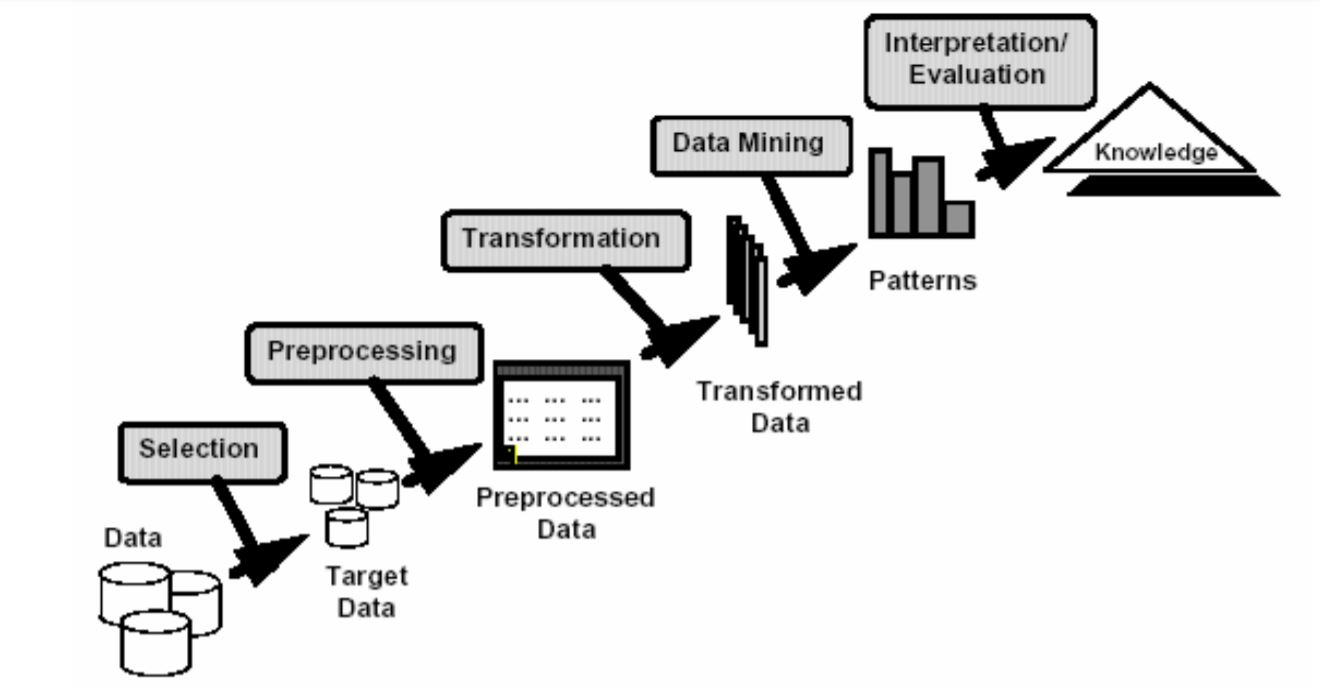
\includegraphics[scale=0.4]{datamining1}
	\caption{Tahapan pada KDD}
	\label{fig:datamining1}
\end{figure}

\noindent Berikut ini adalah penjelasan tahapan pada KDD pada Gambar \ref{fig:datamining1} sebagai berikut:

\begin{enumerate}
\item \textit{Selection}: proses mengambil data yang relevan terhadap analisis.
\item \textit{Preprocessing}: proses pembersihan data dari data yang tidak konsisten dan integrasi data saat penggabungan data.
\item \textit{Transformation}: proses manipulasi data menggunakan konsep agregasi, generalisasi, normalisasi, dan reduksi untuk kebutuhan analisis.
\item \textit{Data mining}: proses ekstraksi informasi menggunakan metode pengenalan pola seperti klasifikasi, pengelompokan/\textit{clustering}.
\item \textit{Interpretation/evaluation}: proses interpretasi hasil pengolahan data menjadi sebuah grafik yang dapat dimengerti.
\end{enumerate}


\noindent Berikut adalah beberapa jenis tipe data terkait teknik data mining:

\begin{itemize}

\item \textit{Binary}: tipe data alphabet/numerik yang hanya memiliki 2 kemungkinan nilai. \\ Contoh: nilai true/false dan 0/1.

\item \textit{Nominal}: tipe data alphabet/numerik yang memiliki lebih dari 2 kemungkinan nilai.\\ Contoh: warna  kuning, hijau, hitam, merah.

\end{itemize}

\noindent Tujuan dari penggunaan teknik \textit{data mining} adalah sebagai berikut:

\begin{itemize}

\item Prediksi: proses menggunakan nilai dari beberapa atribut yang sudah ada untuk memprediksi nilai atribut di masa yang akan datang. Contoh: klasifikasi.

\item Deskripsi: proses menemukan pola yang dapat merepresentasikan kelompok dari sebuah data. Contoh: \textit{clustering}.

\end{itemize}

\subsection{Klasifikasi} 
Klasifikasi adalah proses menemukan model (atau fungsi) yang cocok untuk mendeskripsikan dan membedakan sebuah kelas data dengan kelas data lain. Dalam pembelajaran mesin, klasifikasi sering dianggap sebagai contoh dari metode pembelajaran yang diawasi, yaitu menyimpulkan fungsi dari data pelatihan berlabel.\\

\noindent Berikut adalah tahapan klasifikasi secara umum:
\begin{enumerate}

\item
Pelatihan: proses konstruksi model klasifikasi menggunakan algoritma tertentu. Algoritma digunakan untuk membuat model belajar menggunakan set pelatihan data yang tersedia. Model dilatih untuk menghasilkan prediksi yang akurat.

\item
Klasifikasi: model yang digunakan untuk memprediksi label kelas dan menguji model yang dibangun pada data uji dan karenanya memperkirakan akurasi aturan klasifikasi.
\end{enumerate}
\vspace{0.3cm}
\noindent Berikut adalah kategori pemodelan klasifikasi:
\begin{itemize}

\item 
\textit{Discriminative}: pemodelan paling mendasar untuk menentukan satu kelas untuk setiap baris data. Pemodelan ini bergantung pada data yang diamati dan sangat bergantung pada kualitas data daripada distribusi data.

\begin{figure}[H]
	\centering
	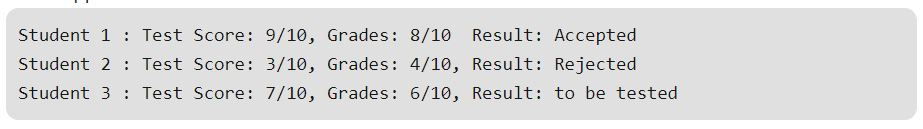
\includegraphics[scale=0.75]{klasifikasi1}
	\caption{Contoh \textit{Logistic Regression}}
	\label{fig:klasifikasi1}
\end{figure}

Contoh: \textit{Logistic Regression}\\
Gambar \ref{fig:klasifikasi1} adalah penerimaan siswa pada sebuah Universitas, untuk mempertimbangkan \textit{test score} dan \textit{grades} terhadap keputusan seorang siswa diterima/tidak diterima.

\item 
\textit{Generative}: pemodelan ini memodelkan distribusi kelas individu dan mencoba mempelajari model yang menghasilkan data dengan memperkirakan asumsi dan distribusi model. Digunakan untuk memprediksi nilai data yang belum diketahui. \\\\
Contoh: \textit{Naive Bayes} \\
Mendeteksi email spam dengan melihat data sebelumnya. Misalkan dari 100 email yang ada dibagi menjadi kategori Kelas A: 25\% (Email spam) dan Kelas B: 75\% (Email Non-Spam). Ingin diperiksa apakah email berisi  spam atau bukan. Pada Kelas A, 20 dari 25 email adalah spam dan sisanya bukan spam. Pada Kelas B, 70 dari 75 email bukan spam dan sisanya adalah spam. Probabilitas email yang berisi spam termasuk pemodelan \textit{Naive Bayes}. \\
\end{itemize}

\noindent Berikut adalah contoh pemodelan klasifikasi yang umum digunakan:
\begin{itemize}
\item \textit{Decision Trees}
\item \textit{Naive Bayes}
\item \textit{Neural Networks}
\item \textit{K-Nearest Neighbour}
\item \textit{Linear Regression}
\end{itemize}

\subsection{\textit{Naive Bayes}}
\label{sec:naive_bayes}
\par \textit{Naive Bayes} menerapkan klasifikasi dengan menggunakan metode probabilitas dan statistik. Pemodelan ini mencari nilai probabilitas tertinggi pada masing-masing kelas menggunakan teorema \textit{Bayes}. Kelas dengan probabilitas tertinggi akan dipilih sebagai hasil akhir. \textit{Naive Bayes} mudah untuk dibangun dan memiliki komputasi yang lebih cepat daripada model klasifikasi lainnya.\\

\noindent Teorema \textit{Bayes} menemukan probabilitas suatu peristiwa terjadi mengingat probabilitas peristiwa lain yang telah terjadi. Teorema \textit{Bayes} dinyatakan secara matematis melalui persamaan berikut:

\begin{equation}
P(H|D) = \frac{P(D|H) \cdot P(H)}{P(D)}
\end{equation}

\noindent
Dari perhitungan probabilitas teorema \textit{Bayes}, akan dicari kelas dengan probabilitas maksimum. Probabilitas maksimum dapat dinyatakan secara matematis melalui persamaan berikut:

\begin{align}
MAP(H) = max(P(H|D))
\end{align}

\noindent Keterangan:
\begin{itemize}
\item $P(H|D)$ adalah probabilitas posterior apabila diberika hipotesis $H$ dan diketahui data $D$. 
\item $P(D|H)$ adalah probabilitas posterior data $D$ jika hipotesis $h$ adalah benar.
\item $P(H)$ adalah probabilitas hipotesis $h$ adalah benar 
\item $P(D)$ adalah probabilitas data.
\end{itemize}

\vspace{0.3cm}

\noindent Tabel \ref{table:naivedataset} diberikan untuk menggambarkan kondisi cuaca saat bermain golf. Masing-masing data dikategorikan berdasarkan nilai atribut \textit{PlayGolf}, yaitu cocok (\textit{Yes}) atau tidak cocok (\textit{No}). 

\begin{table}[h]
\centering
\caption{Contoh Kasus \textit{PlayGolf}}
\begin{tabular}{|c|c|c|c|c|}
\hline 
Outlook & Temperature & Humidity & Windy & PlayGolf \\ 
\hline 
Rainy & Hot & High & False & No \\ 
\hline 
Rainy & Hot & High & True & No \\ 
\hline 
Overcast & Hot & High & False & Yes \\ 
\hline 
Sunny & Mild & High & False & Yes \\ 
\hline 
Sunny & Cool & Normal & False & Yes \\ 
\hline 
Sunny & Cool & Normal & True & No \\ 
\hline 
Overcast & Cool & Normal & True & Yes \\ 
\hline 
Rainy & Mild & High & False & No \\ 
\hline 
Rainy & Cool & Normal & False & Yes \\ 
\hline 
Sunny & Mild & Normal & False & Yes \\ 
\hline 
Rainy & Mild & Normal & True & Yes \\ 
\hline 
Overcast & Mild & High & True & Yes \\ 
\hline 
Overcast & Hot & Normal & False & Yes \\ 
\hline 
Sunny & Mild & High & True & No \\ 
\hline 
\end{tabular} 
\label{table:naivedataset}
\end{table}

\noindent Berikut adalah pengelompokan nilai berdasarkan dataset yang telah diberikan:

\begin{itemize}

\item 
Vektor fitur\\
Vektor fitur adalah vektor yang mewakili nilai fitur untuk setiap baris dataset. Vektor fitur pada contoh kasus ini terdiri dari atribut \textit{Outlook, Temperature, Humidity, dan Windy}.

\item
Vektor respon\\
Vektor respon adalah nilai prediksi dalam bentuk label kelas untuk setiap baris data. Vektor respon pada contoh kasus ini diwakili oleh atribut \textit{PlayGolf}.

\end{itemize}
\vspace{0.5cm}
\noindent Secara singkat, langkah kerja algoritma \textit{Naive Bayes} dapat dijelaskan sebagai berikut:

\begin{enumerate}
\item Merepresentasikan teorema \textit{Bayes} terhadap vektor fitur.\\
Berdasarkan dataset, teorema \textit{Bayes} dapat diubah seperti berikut:

\begin{equation}
P(y|X) = \frac{P(X|y) \cdot P(y)}{P(X)}
\end{equation}

Di mana $y$ adalah label kelas dan $X$ adalah vektor fitur (dengan ukuran $n$), dinyatakan melalui persamaan berikut:

\begin{equation}
X = (x_1, x_2, x_3, \ldots, x_n)
\end{equation}

Contoh: $X = (Rainy, Hot, High, False), y = No$
\\\\
Diasumsikan teorema \textit{Bayes} saling independen terhadap fitur-fiturnya. Berikut adalah persamaan teorema \textit{Bayes} baru, jika memakai lebih dari satu nilai atribut:

\begin{equation}
P(y|x_1,\ldots,x_n) = \frac{P(x_1|y) P(x_2|y) \ldots P(x_n|y) P(y)}{P(x_1) P(x_2) \ldots P(x_n)}
\end{equation}


\item Menghitung probabilitas nilai dari sebuah atribut.\\
Sebagai contoh, nilai yang dimiliki atribut \textit{Outlook} adalah \textit{\{Sunny,Overcast,Rainy\}}. Tabel \ref{table:probabilitas} berfungsi untuk mencatat frekuensi dan menghitung probabilitas nilai dari atribut \textit{Outlook}.


\begin{table}[h]
\centering
\caption{Tabel Probabilitas pada Atribut \textit{Outlook}}
\vspace{0.2cm}
\begin{tabular}{|c|c|c|c|c|}
\hline 
 & Yes & No & P(Yes) & P(No) \\ 
\hline 
Sunny & 3 & 2 & 3/9 & 2/5 \\ 
\hline 
Overcast & 4 & 0 & 4/9 & 0/5 \\ 
\hline 
Rainy & 2 & 3 & 2/9 & 3/5 \\ 
\hline 
Total & 9 & 5 & 100 & 100 \\ 
\hline 
\end{tabular}
\label{table:probabilitas}
\end{table}


Berikut adalah contoh perhitungan $P(No)$ untuk nilai \textit{Sunny} pada atribut \textit{Outlook}
\begin{align*}
P(No) &= \frac{frekuensi(Sunny \cap No)}{frekuensi(No)} = \frac{2}{5}
\end{align*}

Berikut adalah contoh perhitungan $P(Yes)$ untuk nilai \textit{Sunny} pada atribut \textit{Outlook}
\begin{align*}
P(Yes) = \frac{frekuensi(Sunny \cap Yes)}{frekuensi(Yes)} = \frac{3}{9}
\end{align*}

Perhitungan probabilitas $P(Yes)$ dan $P(No)$ berlaku untuk nilai lainnya pada atribut \textit{Outcast} yaitu \textit{\{Overcast,Rainy\}}, sehingga hasil akhirnya dapat dilihat pada Tabel \ref{table:probabilitas}. 

\newpage
\item Membuat tabel probabilitas untuk atribut lainnya \textit{\{Temperature,Humidity, Windy\}} dengan cara yang sama seperti langkah 2. Hasilnya akan menjadi Tabel \ref{table:probabilitas2}, \ref{table:probabilitas3}, \ref{table:probabilitas4}

\begin{table}[h]
\centering
\caption{Tabel Probabilitas dari Atribut Temperature}
\vspace{0.2cm}
\begin{tabular}{|c|c|c|c|c|}
\hline 
 & Yes & No & P(Yes) & P(No) \\ 
\hline 
Hot & 2 & 2 & 2/9 & 2/5 \\ 
\hline 
Mild & 4 & 2 & 4/9 & 2/5 \\ 
\hline 
Cool & 3 & 1 & 3/9 & 1/5 \\ 
\hline 
Total & 9 & 5 & 100\% & 100\% \\ 
\hline 
\end{tabular}
\label{table:probabilitas2}
\end{table}

\begin{table}[h]
\centering
\caption{Tabel Probabilitas dari Atribut Humidity}
\vspace{0.2cm}
\begin{tabular}{|c|c|c|c|c|}
\hline 
 & Yes & No & P(Yes) & P(No) \\ 
\hline 
High & 3 & 4 & 3/9 & 4/5 \\ 
\hline 
Normal & 6 & 1 & 6/9 & /5 \\ 
\hline 
Total & 9 & 5 & 100 & 100 \\ 
\hline 
\end{tabular}
\label{table:probabilitas3}
\end{table}

\begin{table}[h]
\centering
\caption{Tabel Probabilitas dari Atribut Wind}
\vspace{0.2cm}
\begin{tabular}{|c|c|c|c|c|}
\hline 
 & Yes & No & P(Yes) & P(No) \\ 
\hline 
False & 6 & 2 & 6/9 & 2/5 \\ 
\hline 
True & 3 & 3 & 3/9 & 3/5 \\ 
\hline 
Total & 9 & 5 & 100 & 100 \\ 
\hline 
\end{tabular}
\label{table:probabilitas4}
\end{table}

\item Menghitung probabilitas bersyarat terhadap data baru yang diberikan. \\
Contoh: \textit{today = (Sunny, Hot, Normal, NoWind)}

\begin{align*}
P(Yes|today) &= \frac{P(Sunny|Yes)P(Hot|Yes)P(Normal|Yes)P(NoWind|Yes)P(Yes)}{P(today)} \\
&= \frac{3}{5} \cdot \frac{2}{5} \cdot \frac{1}{5} \cdot \frac{2}{5} \cdot \frac{5}{14} = 0.0068
\end{align*}

\begin{align*}
P(No|today) &= \frac{P(Sunny|No)P(Hot|No)P(Normal|No)P(NoWind|No)P(No)}{P(today)}\\
&= \frac{2}{9} \cdot \frac{2}{9} \cdot \frac{6}{9} \cdot \frac{6}{9} \cdot \frac{9}{14} = 0.0068
\end{align*}


\item Melakukan normalisasi terhadap probabilitas besyarat.

\begin{align*}
P(Yes|today) = \frac{0.0141}{0.0141 + 0.0068} = 0.67
\end{align*}

\begin{align*}
P(No|today) = \frac{0.0068}{0.0141 + 0.0068} = 0.33
\end{align*}

Ketika probabilitas tersebut dijumlahkan, maka hasilnya akan menjadi 1.

\begin{equation}
P(Yes|today) + P(No|today) = 1
\end{equation}

\item Mencari probabilitas tertinggi.\\

Berdasarkan pernyataan berikut:
\begin{equation}
P(Yes|today) > P(No|today)
\end{equation}

\noindent Dapat disimpulkan bahwa data dengan nilai \textit{(Sunny, Hot, Normal, NoWind)} dapat diklasifikasikan terhadap atribut $PlayGolf$ dengan nilai label kelas\textit{Yes}.

\end{enumerate}

\subsection{\textit{Clustering}} 
{\it Clustering} merupakan proses mengelompokkan satu data ke dalam himpunan data yang disebut {\it cluster}. Objek di dalam {\it cluster} memiliki kemiripan karakteristik satu sama lain yang berbeda dengan {\it cluster} lainnya. {\it Clustering} sangat berguna untuk menemukan kelompok data yang tidak dikenal. {\it Clustering} sering disebut juga sebagai {\it outlier detection}. \\

\noindent Berikut adalah tahapan {\it clustering} secara umum:
\begin{enumerate}
\item Perhitungan \textit{distance}: proses untuk mengukur kesamaan antar objek dengan cara menghitung \textit{distance} antar 2 titik. Salah satu contoh metode pengukuran \textit{distance} yang umum digunakan adalah {\it Euclidean distance}. Metode ini terdiri atas variabel $p_i$, menyatakan kordinat titik data dan variabel $C_i$, menyatakan kordinat titik \textit{centroid} sebuah \textit{cluster}.\\

\noindent Berikut adalah persamaan untuk menghitung \textit{Euclidean distance}:
\begin{equation}
EuclidDist(p_i,C_i) = \sqrt[]{(p_1-C_1)^2+(p_2-C_2)^2+\ldots +(p_n-C_n)^2}
\end{equation}

\item Pengelompokan data: proses pencarian anggota \textit{cluster} dengan menghitung \textit{distance} minimum antara masing-masing titik data dengan titik \textit{centroid cluster} tersebut.
\end{enumerate}
\vspace{0.3cm}

\noindent Berikut adalah kategori pemodelan {\it clustering}:
\begin{itemize}
\item \textit{Hierarchical clustering}: pengelompokan data pada sebuah hirarki dengan cara menggabung dua kelompok data terdekat maupun membagi data ke dalam cluster tertentu. Contoh pemodelannya adalah {\it single linkage, complete linkage, average linkage, average group linkage}.

\begin{figure}[H]
	\centering
	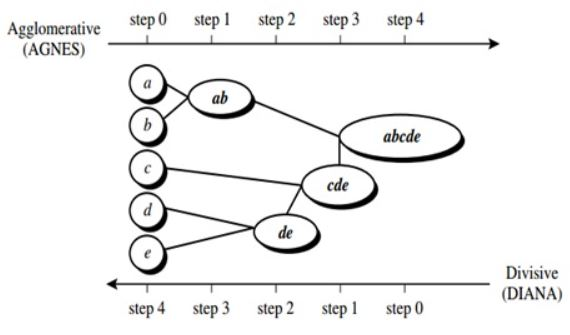
\includegraphics[scale=0.75]{metode_clustering_1}
	\caption{Contoh {\it Hierarchical Clustering}}
	\label{fig:metode_clustering_1}
\end{figure} 

\item \textit{Partitional clustering}: pengelompokan data ke dalam sejumlah \textit{cluster} tanpa adanya struktur hierarki. Pada metode ini, setiap \textit{cluster} memiliki titik pusat cluster (centroid) dengan tujuan untuk meminimumkan ({\it dissimilarity distance}) seluruh data ke {\it centroid cluster} masing-masing. Contoh pemodelannya adalah {\it k-means, fuzzy k-means,} dan {\it mixture modeling}.

\begin{figure}[H]
	\centering
	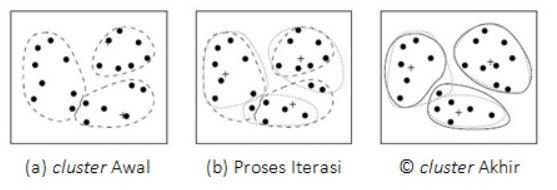
\includegraphics[scale=0.7]{metode_clustering_2}
	\caption{Contoh {\it Partitional Clustering}}
	\label{fig:metode_clustering_2}
\end{figure}

\end{itemize}

\noindent Berikut adalah contoh pemodelan {\it clustering} yang umum digunakan:
\begin{itemize}
\item {\it Agglomerative}
\item {\it K-Means}
\end{itemize}

\subsection{\textit{K-Means}} 
\label{sec:k_means}
\textit {K-means} merupakan metode clustering yang paling sederhana dan umum. {\it K-means} merupakan salah satu algoritma {\it clustering} dengan metode {\it partitional clustering} menggunakan titik {\it centroid} sebagai pusat kelompok data. {\it K-means} memerlukan tiga jenis paramater yaitu menentukan jumlah kelompok data (k),  inisialisasi titik {\it centroid} awal, dan mengetahui {\it distance} antar titik. \\


\noindent Tabel \ref{table:datakmeans} diberikan untuk mengelompokan mata pelajaran yang sejenis berdasarkan data skor yang diperoleh dari individu A dan B:

\begin{table}[h]
\centering
\caption{Tabel Dataset Mata Pelajaran}
\vspace{0.2cm}
\begin{tabular}{|c|c|c|}
\hline 
Subject & Person A & Person B \\ 
\hline 
1 & 1.0 & 1.0 \\ 
\hline 
2 & 1.5 & 2.0 \\ 
\hline 
3 & 3.0 & 4.0 \\ 
\hline 
4 & 5.0 & 7.0 \\ 
\hline 
5 & 3.5 & 5.0 \\ 
\hline 
6 & 4.5 & 5.0 \\ 
\hline 
7 & 3.5 & 4.5 \\ 
\hline 
\end{tabular} 
\label{table:datakmeans}
\end{table}

\noindent Secara singkat, langkah kerja algoritma \textit{k-means} dapat dijelaskan sebagai berikut:
\begin{enumerate}

\item Inisialisasi k dan titik {\it centroid} awal. \\
Pada contoh ini, jumlah {\it cluster} yang ingin dibentuk adalah dua kelompok data atau $k = 2$ dengan inisialisasi titik {\it centroid} awal adalah $(1.0,1.0)$ dan $(5.0,7.0)$. Kedua titik ini dipilih secara acak. Data ini direpresentasikan pada Tabel \ref{table:kmeans_2} seperti berikut.

\begin{table}[h]
\centering
\caption{Hasil Pengelompokan Awal}
\vspace{0.2cm}
\begin{tabular}{|c|c|C{2cm}|}
\hline 
 & Individual & Centroid \\ 
\hline 
Cluster 1 & 1 & (1.0, 1.0) \\ 
\hline 
Cluster 2 & 4 & (5.0, 7.0) \\ 
\hline 
\end{tabular}
\label{table:kmeans_2}
\end{table} 

\newpage
\item Melakukan perhitungan {\it distance}.\\
{\it Distance} digunakan untuk mencari jarak antara sebuah titik data dengan titik {\it centroid} dari {\it cluster} tertentu. Sebagai contoh, \textit{distance} antara data ke-1 $(1.5,2.0)$ dengan titik {\it centroid} dari {\it Cluster 1} $(1.0,1.0)$ dihitung menggunakan {\it Euclidean distance} sebagai berikut.

\begin{align*}
EuclidDist(p_i,C_i) &= \sqrt[]{(p_1-C_1)^2+(p_2-C_2)^2+\ldots +(p_n-C_n)^2} \\
&= \sqrt[]{(1.5-1.0)^2+(2.0-1.0)^2} = 1.1180
\end{align*}

\item Menempatkan setiap titik data ke titik {\it centroid} terdekat.\\
Titik data akan dikelompokan ke {\it centroid} terdekat dengan memilih nilai Euclidian {\it distance} paling kecil. Sebagai contoh, Tabel \ref{table:kmeans_3} pada {\it Step 2} menyatakan data ke-1 lebih dekat dengan data ke-2, karena memiliki nilai Euclidean distance paling kecil. Karena itu, data ke-2 bergabung pada titik {\it centroid} data ke-1. Hal ini berlaku pada setiap langkah. 

\begin{table}[h]
\centering
\caption{Mencari Centroid Kelompok}
\vspace{0.2cm}
\begin{tabular}{|c|c|C{2cm}|c|C{2cm}|}
\hline 
 & \multicolumn{2}{c|}{Cluster 1} &   \multicolumn{2}{c|}{Cluster 2}  \\ 
\hline 
Step & Individual & Mean Vector (centroid) & Individual & Mean Vector (centroid) \\ 
\hline 
1 & 1 & (1.0, 1.0) & 4 & (5.0, 7.0) \\ 
\hline 
2 & 1, 2 & (1.2, 1.5) & 4 & (5.0, 7.0) \\ 
\hline 
3 & 1, 2, 3 & (1.8, 2.3) & 4 & (5.0, 7.0) \\ 
\hline 
4 & 1, 2, 3 & (1.8, 2.3) & 4, 5 & (4.2, 6.0) \\ 
\hline 
5 & 1, 2, 3 & (1.8, 2.3) & 4, 5, 6 & (4.3, 5.7) \\ 
\hline 
6 & 1, 2, 3 & (1.8, 2.3) & 4, 5, 6, 7 & (4.1, 5.4) \\ 
\hline 
\end{tabular} 
\label{table:kmeans_3}
\end{table}

\noindent Setelah pengelompokan data selesai dilakukan, selanjutnya perlu menghitung {\it Mean Vector (centroid)} sebagai titik {\it centroid} baru sebuah {\it cluster}. Sebagai contoh, {\it Mean Vector} pada {\it Cluster 1} untuk {\it Step 2} dapat dihitung sebagai berikut.

\begin{align*}
MeanVector(Person A) &= \frac{1.0+1.5}{2} = 1.2 \\
MeanVector(Person B) &= \frac{1.0+2.0}{2} = 1.5
\end{align*}

\item Menetapkan kelompok data baru pada masing-masing {\it cluster}.\\
Iterasi paling terakhir di langkah sebelumnya akan dijadikan sebagai anggota dari {\it cluster} baru. Tabel \ref{table:kmeans_4} menunjukan kelompok data sementara yang terbentuk pada masing-masing {\it cluster}. {\it Cluster 1} terdiri dari anggota data $\{1,2,3\}$, sedangkan {\it Cluster 2} terdiri dari anggota data $\{4,5,6,7\}$. Kelompok data yang terbentuk saat ini masih sementara dan dapat berubah-ubah.

\begin{table}[h]
\centering
\caption{Hasil Cluster Baru}
\vspace{0.2cm}
\begin{tabular}{|c|c|C{2cm}|}
\hline 
 & Individual & Mean Vector (centroid) \\ 
\hline 
Cluster 1 & 1, 2, 3 & (1.8, 2.3) \\ 
\hline 
Cluster 2 & 4, 5, 6, 7 & (4.1, 5.4) \\ 
\hline 
\end{tabular} 
\label{table:kmeans_4}
\end{table} 

\item Mencari titik {\it centroid} baru untuk setiap {\it cluster}.\\
Belum dipastikan bahwa setiap individu telah dialokasikan dengan tepat. Oleh karena itu, langkah 1 sampai 4 perlu kembali diulang dengan menghitung kembali \textit{Euclidean distance}. Tabel \ref{table:kmeans_5} merupakan hasil perhitungan {\it distance} untuk setiap titik data.

\begin{table}[h]
\centering
\caption{Euclidean Distance Cluster 1, Cluster 2}
\vspace{0.2cm}
\begin{tabular}{|c|C{2cm}|C{2cm}|}
\hline 
Individual & Distance centroid  of Cluster 1 & Distance centroid  of Cluster 2 \\ 
\hline 
1 & 1.5 & 5.4 \\ 
\hline 
2 & 0.4 & 4.3 \\ 
\hline 
3 & 2.1 & 1.8 \\ 
\hline 
4 & 5.7 & 1.8 \\ 
\hline 
5 & 3.2 & 0.7 \\ 
\hline 
6 & 3.8 & 0.6 \\ 
\hline 
7 & 2.8 & 1.1 \\ 
\hline 
\end{tabular} 
\label{table:kmeans_5}
\end{table} 

\item Menetapkan kelompok data akhir.\\
Apabila {\it cluster} tidak mengalami perubahan secara signifikan pada anggotanya selama periode iterasi tertentu, maka {\it cluster} yang terbentuk sudah sesuai. Tabel \ref{table:kmeans_6} menunjukan anggota dari {\it cluster} yang sudah tetap, sehingga proses {\it k-means} dapat dihentikan.

\begin{table}[h]
\centering
\caption{Hasil Pengelompokan Akhir}
\vspace{0.2cm}
\begin{tabular}{|c|c|C{2cm}|}
\hline 
 & Individual & Mean Vector (centroid) \\ 
\hline 
Cluster 1 & 1, 2 & (1.3, 1.5) \\ 
\hline 
Cluster 2 & 3, 4, 5, 6, 7 & (3.9, 5.1) \\ 
\hline 
\end{tabular}
\label{table:kmeans_6}
\end{table} 

\end{enumerate}

\section{Tahapan Evaluasi \textit{Data Mining}}
Setelah melakukan implementasi model {\it data mining}, langkah selanjutnya adalah mengevaluasi hasil dari model {\it data mining} yang telah dibuat. Tahapan evaluasi sangat penting untuk mengukur seberapa tinggi tingkat akurasi model yang dipilih untuk menyelesaikan sebuah permasalahan data. Metode evaluasi untuk setiap model {\it data mining} berbeda satu sama lain. Oleh karena itu, perlu untuk mendefinisikan perhitungan evaluasi untuk masing-masing model. 

\subsection{Menghitung Tingkat Akurasi untuk Model Klasifikasi}
Hasil pemodelan klasifikasi dapat dievaluasi menggunakan perhitungan tingkat akurasi. Semakin tinggi tingkat akurasi yang diperoleh, maka hasil pemodelan klasifikasi menjadi semakin baik. Akurasi dihitung dari rasio jumlah prediksi yang benar dengan jumlah total sampel input. \\

\noindent Berikut adalah persamaan untuk menghitung tingkat akurasi:
\begin{align}
Tingkat\:Akurasi = \frac{jumlah\:prediksi\:yang\:benar}{total\:sampel\:input} \times 100\%
\end{align}

\noindent Kisaran skor untuk tingkat akurasi adalah $[\:0\%,100\%\:]$.

\subsection{Menghitung Koefisien \textit{Silhouette} untuk Model \textit{Clustering}}
Hasil pemodelan {\it clustering} dapat dievaluasi menggunakan perhitungan koefisien {\it silhouette}. Koefisien {\it silhouette} bertujuan untuk menghitung seberapa dekat sebuah objek dengan {\it intra-cluster} dan mengukur seberapa jauh objek yang sama dengan {\it cluster} terdekat lainnya. Semakin tinggi nilai koefisien {\it silhouette}, maka hasil pengelompokannya akan semakin baik. Koefisien {\it silhouette} dihitung berdasarkan rata-rata {\it distance} antara setiap titik data dengan titik {\it centroid intra-cluster} dan  rata-rata {\it distance} antara setiap titik data dengan titik {\it centroid cluster} lainnya.\\


\noindent Kisaran skor koefisien {\it silhouette} adalah $[\:-1, 1\:]$, berikut adalah analisisnya:
\begin{itemize}
\item Skor 1, artinya sampel berada jauh dari {\it cluster} tetangganya.
\item Skor 0, artinya bahwa sampel sangat dekat dengan {\it cluster} tetangganya
\item  Skor -1, artinya sampel telah dikelompokan pada {\it cluster} yang salah.
\end{itemize}

\vspace{0.3cm}
\noindent Berikut adalah persamaan untuk menghitung koefisien {\it silhouette}:
\begin{align}
Silhouette\:Score = \frac{(p\:-\:q)}{max(p,q)}
\end{align}

\noindent Keterangan:
\begin{itemize}
\item $p$ = rata-rata {\it distance} setiap titik {\it intra-cluster} terhadap titik {\it centroid} pada {\it cluster} terdekat.
\item $q$ = rata-rata {\it distance} setiap titik {\it intra-cluster} terhadap titik {\it centroid intra-cluster}.
\item $max(p,q)$ = nilai maksimum dari $p$ dan $q$.
\end{itemize}



\section{\textit{Privacy-Preserving Data Mining} (PPDM)} 

Di era informasi saat ini, sistem informasi terus menghasilkan banyak informasi. Namun, banyak dari informasi yang dikumpulkan bersifat sensitif seperti data pribadi yang dapat menimbulkan masalah privasi. Untuk melindungi kebocoran informasi, metode preservasi privasi telah dikembangkan untuk melindungi entitas pemilik data dengan memodifikasi data asli menjadi data yang disamarkan atau data anonim. Akan tetapi metode ini memiliki kekurangan karena secara tidak langsung mengubah isi data, sehingga informasi yang didapat menjadi berkurang. Hal ini mengakibatkan ekstraksi informasi melalui proses {\it data mining} menjadi tidak akurat. 

\textit{Privacy Preserving Data Mining} (PPDM) adalah metodologi yang dirancang khusus untuk menjamin tingkat privasi pada level tertentu, sekaligus memaksimalkan  utilitas data saat dilakukan proses data mining. PPDM mencakup semua teknik yang dapat digunakan untuk mengekstrak pengetahuan dari data dan secara bersama menjaga privasi dari data tersebut. Menurut IEEE, metodologi ini dapat dibagi menjadi beberapa bagian yaitu metode perlindungan privasi dan metrik perlindungan privasi yang akan dijelaskan pada bagian selanjutnya.

\textit Gambar \ref{fig:ppdm} menjelaskan garis besar pokok pembahasan dari PPDM yaitu metode, metrik, dan bidang penerapannya. Metode PPDM dapat diterapkan fase siklus data mulai dari pengumpulan data, publikasi data, hasil {\it data mining}, sampai kepada distribusi data. Selain itu, PPDM juga memiliki metrik untuk mengevaluasi dan membandingkan teknik-teknik yang digunakan agar mencapai tingkat privasi dan kualitas data tertentu. PPDM umumnya diaplikasikan pada bidang {\it cloud computing, e-health, wireless sensor,} dan {\it location-based service}.

\begin{figure}[H]
	\centering
	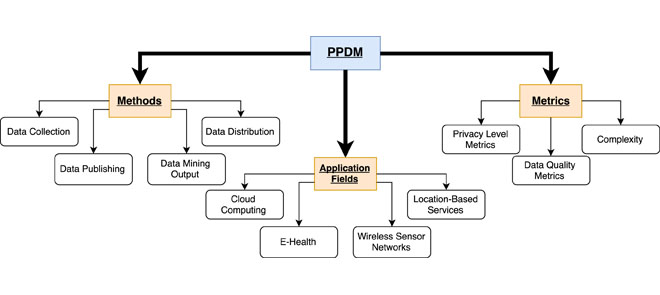
\includegraphics[scale=2.5]{ppdm}
	\caption{\textit{Privacy Preserving Data Mining} (PPDM)}
	\label{fig:ppdm}
\end{figure}

\subsection{Metode pada PPDM}

Beberapa metode PPDM telah diusulkan untuk menjamin perlindungan privasi pada masing-masing fase siklus hidup sebuah data di mana fase siklus tersebut sering terjadi pelanggaran privasi saat pengumpulan data, penerbitan data, distribusi data dan terhadap hasil {\it data mining}. \\ 

\noindent Berikut adalah metode perlindungan privasi pada PPDM:

\begin{itemize}	

\item Pengumpulan data\\
Pada fase ini, entitas yang bertugas mengumpulkan data tidak dapat dipercaya karena dapat mengumpulkan dan menggunakan data privasi individu secara tidak benar. Metode yang dapat digunakan untuk melindungi privasi saat pengumpulan data adalah {\it randomisation}.

\item Publikasi data\\
Pada fase ini, entitas ingin mempublikasikan datanya untuk keperluan penelitian atau analisis. Akan tetapi, ada beberapa individu yang mencoba melakukan tindakan deanonimisasi pada data-data privasi milik seseorang untuk tindakan kejahatan. Metode yang dapat digunakan untuk melindungi privasi saat publikasi data adalah {\it k-anonymity}.

\item Hasil data mining\\
Hasil data mining biasanya dibuat mudah diakses melalui aplikasi atau {\it interface}. Pada fase ini, entitas dapat melakukan kueri pada sistem untuk mencari informasi sensitif seseorang. Metode yang dapat digunakan untuk melindungi privasi pada hasil data mining adalah {\it association rule hiding, downgrading classifier effectiveness,} dan {\it query auditing and inference control}.

\item Distribusi data\\
Pada fase ini, beberapa entitas akan mencari wawasan umum dalam bentuk data statistik tanpa mengungkap informasi entitas lain. Akan tetapi ada beberapa entitas yang sengaja  untuk menemukan celah keamanan privasi melalui pencocokan data dengan informasi umum yang diberikan secara publik. Hal ini dapat dicegah dengan memberlakukan {\it multiparty protocol} pada sistem distribusi data.

\end{itemize}

\subsection{Metrik pada PPDM}
Karena privasi tidak memiliki standar definisi yang jelas, maka diperlukan metrik untuk mengukur keamanan privasi. Melalui metode PPDM, beberapa metrik perlindungan privasi telah diusulkan. Metrik PPDM terbagi menjadi dua kategori utama yaitu privasi data dan kualitas data. \\

\noindent Berikut adalah metrik perlindungan privasi pada PPDM:

\begin{itemize}

\item Tingkatan Privasi \\
Tingkatan privasi memberikan gambaran seberapa aman data diolah agar terhindar dari kasus pelanggaran privasi . Metrik ini dapat ditemukan pada model {\it k-anonymity}. Model k-anonymity berpengaruh terhadap tingkat privasi, dimana nilai $k$ dapat diubah sesuai keinginan dalam menentukan tingkat keamanan data.

\item Kualitas Data\\
Kualitas data dinilai dari tiga parameter penting. {\it Accuracy}, untuk mengukur seberapa dekat nilai data yang disamarkan dengan data asli. {\it Completeness}, untuk mengevaluasi banyaknya data yang hilang. {\it Consistency}, untuk mengukur hilangnya korelasi data pada data yang disamarkan. Pada pemodelan {\it k-anonymity}, metrik yang dapat diukur untuk menyatakan kualitas data adalah {\it Information Loss} (IL).

\end{itemize}

\subsection{Model Serangan pada PPDM}
Menurut Dalenius (1977), perlindungan privasi tidak memberikan kesempatan bagi orang lain untuk mendapatkan informasi sensitif individu meskipun orang lain mengetahui informasi umum yang berhubungan dengan informasi sensitif individu tersebut. Secara umum, orang lain dapat menemukan sebuah cara untuk memetakan sebuah data ke dalam tabel yang telah dianonimisasi ketika data tersebut telah dipublikasi. Serangan ini dikenal dengan istilah \textit{linkage attack}. \\

\noindent Berikut adalah jenis serangan dari \textit{linkage attack}:

\begin{itemize}

\item \textit{Record Linkage}\\
\textit{Record Linkage} mengacu serangan mencocokan antara rekord korban yang dirilis dengan record korban yang telah diketahui untuk menebak atribut sensitif milik korban. Jika record tersebut cocok dengan record lain, artinya kedua data saling berkaitan. Serangan ini dapat dicegah dengan penggunaan model {\it k-anonymity}.
 
\item \textit{Attribute Linkage}\\
\textit{Attribute Linkage} mengacu serangan untuk mendapatkan beberapa informasi  nilai atribut sensitif korban dengan mencari keterhubungan atribut. Tipe serangan ini  mencari keterhubungan nilai atribut non sensitif untuk menebak atribut sensitif milik korban. Serangan ini dapat dicegah dengan penggunaan model {\it l-diversity}.

\end{itemize}

\section{Anonimisasi}
\label{sec:anonimisasi}

Anonimisasi data mengacu pada penghapusan atau enkripsi informasi pribadi atau data sensitif. Karena bisnis, pemerintah, sistem perawatan kesehatan, dan organisasi lain semakin banyak menyimpan informasi individu di server lokal atau cloud, anonimisasi data sangat penting untuk menjaga integritas data dan mencegah pelanggaran keamanan.Di sektor kesehatan dan keuangan, data dapat menjadi hal yang sangat sensitif. Data pasien atau entitas lain harus disembunyikan untuk memenuhi persyaratan perlindungan privasi.

Anonimisasi berupaya melindungi data pribadi atau atribut sensitif dengan menghapus atau mengenkripsi informasi yang dapat diidentifikasi secara pribadi dari database. Anonimisasi data dilakukan dengan tujuan melindungi aktivitas pribadi individu atau perusahaan sambil menjaga integritas data yang dikumpulkan dan dibagikan. Teknik anonimisasi data juga dikenal sebagai {\it "obfuscation data", "data masking"}. Sedangkan {\it data de-anonymization} merupakan teknik yang digunakan pada proses {\it data mining} dengan tujuan untuk mengidentifikasi kembali informasi yang hilang pada data yang dienkripsi atau dianonimisasi.

\section{\textit{K-Anonymity}}
\textit{K-anonymity} merupakan model yang paling efektif untuk melindungi privasi saat melakukan publikasi data. \textit{K-anonymity} adalah contoh pemodelan dari keamanan informasi yang bertujuan agar sebuah data tidak dapat dibedakan setidaknya dengan $k-1$ data lainnya. Dengan kata lain, penyerang tidak dapat mengidentifikasi identitas dari satu data karena $k-1$ data yang lain memiliki sifat yang sama. Dalam pemodelan {\it k-anonymity}, nilai $k$ dapat digunakan sebagai tingkat keamanan privasi. Semakin tinggi nilai $k$, semakin sulit untuk mengindentifikasi sebuah data. Secara teori, probabilitas identifikasi sebuah data adalah $1\;/\;k$. Namun, peningkatan nilai $k$ juga dapat berpengaruh terhadap nilai informasi yang diperoleh dari sekumpulan data.

\par Penelitian menunjukkan bahwa sebagian besar pemodelan \textit{k-anonymity} menggunakan metode generalisasi dan supresi. Pendekatan tersebut menderita kehilangan informasi yang signifikan karena mereka sangat bergantung terhadap hubungan relasi antar atribut. Oleh karena itu, hasil anonimisasi menghasilkan nilai kehilangan informasi yang cukup tinggi. Selain itu, algoritma anonimisasi yang ada hanya berfokus pada perlindungan informasi pribadi dan mengabaikan utilitas data yang sebenarnya. Akibatnya, nilai utilitas pada data yang telah dianonimisasi memiliki nilai yang rendah. Beberapa algoritma telah diuji pada pemodelan \textit{k-anonymity}.\\

\noindent Berikut algoritma yang dapat diterapkan pada pemodelan \textit{k-anonymity}:

\begin{itemize}

\item Algoritma \textit{k-means clustering} akan melakukan beberapa iterasi sampai \textit{centroid} dari semua data tidak lagi berubah atau perubahannya kecil. Algoritma \textit{k-means clustering} tidak mampu untuk menyelesaikan masalah pada atribut yang bernilai kategorikal. Kelebihan dari algoritma \textit{k-means clustering} adalah memiliki hasil pengelompokan yang sudah baik. Kekurangan dari algoritma \textit{k-means clustering} adalah pemilihan {\it centroid} awal {\it k-means} secara acak, sehingga setelah digeneralisasi hasil pengelompokannya mengakibatkan hilangnya informasi yang besar.

\item Algoritma \textit{k-member} dapat melakukan generalisasi atribut kategorikal dengan memperoleh kualitas informasi yang lebih baik daripada algoritma \textit{k-means clustering}. Namun algoritma \textit{k-member} masih memiliki masalah ketika melakukan pengelompokan data. Kekurangan dari algoritma \textit{k-member} adalah hanya mempertimbangkan pengelompokan data pada baris yang terakhir tanpa memperhatikan pengelompokan yang dihasilkan pada proses sebelumnya sehingga menyebabkan distribusi kelompok data pada beberapa bagian menjadi kurang tepat. 

\item Untuk menghindari kekurangan pada algoritma \textit{k-means} dan algoritma \textit{k-member}, maka kedua pendekatan ini digabung menjadi algoritma baru yaitu  \textit{Greedy k-member clustering}. Algoritma \textit{Greedy k-member clustering} mendapatkan hasil pengelompokan yang lebih tepat dan memiliki nilai informasi yang lebih baik meskipun dilakukan generalisasi. Hasil akhir dari algoritma \textit{Greedy k-member clustering} adalah data-data yang sejenis telah dikelompokan pada kelompok data yang sama. Untuk melakukan anonimisasi, digunakan konsep \textit{Hierarchy Based Generalization}. \textit{K-anonymity} menyamarkan data pada nilai quasi-identifier yang sama. 

\end{itemize}

\noindent Berikut adalah atribut dari pemodelan \textit{k-anonymity}, yaitu:
 
\begin{itemize}
\item \textit{Identifier} (ID) adalah atribut yang unik dan secara langsung dapat mengidentifikasi seseorang seperti nama, nomor ID, dan nomor ponsel.
\item \textit{Quasi-identifier} (QID) adalah kombinasi atribut yang mungkin terjadi untuk mengidentifikasi individu berdasarkan penggabungan informasi lain dari luar. Seluruh atribut data terkecuali atribut identifier dapat dianggap sebagai atribut quasi-identifier.
\item \textit{Sensitive Attribute} (SA) adalah atribut yang menyangkut informasi  sensitif seseorang, biasanya nilai atribut ini akan dirahasiakan saat distribusi data.
\item \textit{Non-sensitive Attribute} (NSA) adalah atribut yang tidak menyangkut informasi sensitif seseorang, biasanya nilai atribut ini langsung ditampilkan saat distribusi data.
\end{itemize}

\section{\textit{Hierarchy Based Generalization}} 
\label{theory:hierarchy_generalization}
\textit{Hierarchy-based generalization} adalah tahapan anonimisasi pada pemodelan k-anonymity dimana \textit{quasi-identifier} yang sama dikelompokan ke dalam cluster yang sama. \textit{Hierarchy-based generalization} menggunakan konsep generalisasi dan supresi dalam melakukan anonimisasi. \textit{Hierarchy-based generalization} termasuk metode \textit{full-domain generalization}. \textit{Full-domain generalization} diusulkan oleh Samarati dan Sweeney untuk memetakan seluruh domain untuk masing-masing atribut \textit{quasi-identifier} pada tabel ke domain yang lebih umum berdasarkan kategori tertentu.

\textit{Full-domain generalization} dapat digunakan oleh model \textit{k-anonymity} untuk menentukan generalisasi dan supresi dari sebuah nilai. \textit{Full-domain generalization} menetapkan bahwa proses anonimisasi data dapat dilakukan dengan metode generalisasi apabila atribut \textit{quasi-identifier} telah dipilih sejak awal. Sebagai contoh, dipilih atribut quasi-identifier sebagai berikut $QI = \{A_1,\;\ldots ,\;A_n\}$, dimana A adalah atribut pada tabel dataset. Terdapat dua jenis hierarki pada \textit{Full-domain generalization}, yaitu Domain Generalization Hierarchy (DGH) dan \textit{Value Generalization Hierarchy (VGH)}. Jenis hierarki yang paling umum digunakan adalah DGH. DGH merupakan konsep sederhana dari penggantian nilai berdasarkan nilai yang kurang spesifik menjadi nilai lebih umum terhadap nilai aslinya. Tidak terdapat aturan khusus untuk memodelkan hierarki DGH. Beberapa nilai atribut harus digeneralisasi menggunakan DGH untuk mengakhiri proses anonimisasi data. 

Pada Gambar \ref{fig:DGH1}, nilai ZIP \{02138, 02139\} dapat digeneralisasi menjadi $\{0213*\}$ dengan menghilangkan digit paling kanan. Nilai yang telah digeneralisasi akan memiliki lingkup nilai yang lebih besar. Sebagai contoh, nilai $ZIP$ adalah $\{02138, 02139\}$ berada pada domain dasar yaitu $Z_0$. Untuk mencapai perlindungan data pada \textit{k-anonymity}, maka kode $ZIP$ yang sebelumnya unik harus diubah menjadi bentuk umum. Sebuah nilai dapat digeneralisasi jika memiliki domain yang lebih umum. Sedangkan domain yang kurang spesifik digunakan untuk mendeskripsikan garis besar nilai ZIP. Sebagai contoh dari domain kurang spesifik adalah $Z_1$, di mana digit terakhir diganti dengan simbol (*). Berikut contoh pemetaan dari $Z0$ ke $Z1$ seperti berikut $02139 \rightarrow 0213*$.

Representasi generalisasi dapat diperluas, agar metode supresi dapat diterapkan dalam hirarki generalisasi. Elemen baru dengan nilai supresi maksimal $(*****)$ memiliki posisi lebih tinggi dibandingkan dengan elemen generalisasi $(021**)$. Ketinggian setiap hierarki generalisasi akan bertambah seiring bertambahnya kategori elemen generalisasi. Setelah elemen mencapai nilai supresi maksimal yang dapat digeneralisasi $(*****)$, maka tidak akan ada lagi perubahan yang diperlukan untuk memasukkan elemen generalisasi yang baru. Gambar \ref{fig:DGH1} dan \ref{fig:DGH2} adalah contoh hierarki generalisasi DGH dan VGH pada atribut $ZIP$ (kode pos) dan $Race$ (warna kulit).

\begin{figure}[H]
	\centering
	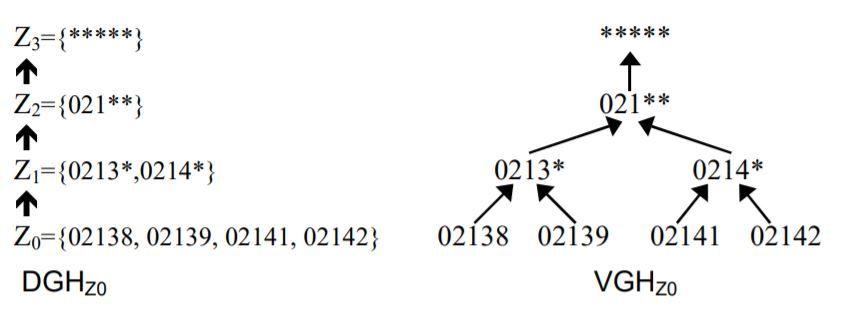
\includegraphics[scale=0.5]{DGH1}
	\caption{DGH dan VGH pada Atribut ZIP}
	\label{fig:DGH1}
\end{figure}

\begin{figure}[H]
	\centering
	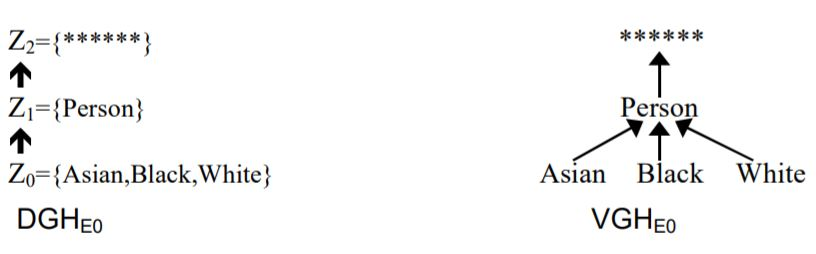
\includegraphics[scale=0.5]{DGH2}
	\caption{DGH dan VGH pada Atribut Race}
	\label{fig:DGH2}
\end{figure}


\section{\textit{Greedy K-Member Clustering}}
\label{sec:greedyclustering}
Sebagian besar metode \textit{k-anonymity} memakai metode generalisasi dan supresi sehingga data menderita kehilangan informasi yang signifikan. Masalah pengelompokan dipercaya dapat meminimalkan kehilangan informasi melalui implementasi algoritma \textit{k-member clustering}. Akan tetapi algoritma tersebut memiliki kompleksitas eksponensial $O(2^n)$, sehingga perlu ditransformasi dengan algoritma \textit{Greedy} dengan kompleksitas $O(n log n)$. Algoritma \textit{Greedy k-member clustering} bertujuan melakukan pengelompokan data ke masing-masing \textit{cluster} dengan kompleksitas algoritma yang lebih baik dan dapat meminimalkan nilai informasi yang hilang saat dilakukan anonimisasi data.

\vspace{0.3cm}
\begin{theorem}
Masalah pengambilan keputusan pada \textit{k-member clustering} adalah \textit{NP-Hard}. \textit{NP-Hard} adalah suatu kelompok masalah dimana tidak ada algoritma yang dapat menemukan solusi optimal dengan kompleksitas lebih kecil dari polinomial.
\end{theorem}

\begin{proof}
Melalui percobaan Aggarwal et al dengan model \textit{3-anonymity}, telah dibuktikan bahwa satu-satunya cara untuk melakukan anonimisasi atribut, yaitu dengan cara melakukan iterasi dari node paling atas (\textit{root node}) ke node paling bawah (\textit{leaf node}).
\end{proof}

\begin{theorem}
N adalah total data dan k adalah parameter untuk anonimisasi. Setiap \textit{cluster} yang ditemukan oleh algoritma \textit{Greedy k-member clustering} memiliki jumlah tuple minimal sebanyak k, dan jumlah tuple tidak melebihi $2k - 1$.
\end{theorem}

\begin{proof}
S adalah himpunan data. Algoritma ini menemukan \textit{cluster} selama jumlah data yang tersisa sama dengan atau lebih besar dari k, setiap \textit{cluster} berisi k data. Jika total data pada S kurang dari k, maka sisa data akan dikelompokan pada  \textit{cluster} yang sudah ada. Oleh karena itu, ukuran maksimum sebuah \textit{cluster} adalah $2k - 1$.
\end{proof}

\begin{theorem}
N adalah jumlah data dan k menjadi parameter anonimisasi yang ditentukan. Jika $n > k$, kompleksitas algoritma \textit{Greedy k-member clustering} adalah $O(n^2)$.
\end{theorem}

\begin{proof}
Algoritma \textit{Greedy k-member clustering} menghabiskan sebagian besar waktunya untuk memilih data dari S satu per satu hingga mencapai $|S| = k$. Karena ukuran set input berkurang satu pada setiap iterasi, total waktu eksekusi adalah O $(n^2)$.
\end{proof}

\vspace{0.5cm}
\noindent Beberapa hal penting terkait algoritma \textit{Greedy k-means clustering}:

\begin{itemize}
\item Menetapkan tabel S  
\item Menetapkan nilai k
\item Menetapkan jumlah cluster (m) yang ingin dibuat
\begin{align}
m = \left \lfloor \frac{n}{k} \right \rfloor - 1
\end{align}
\end{itemize}

\vspace{0.5cm}
\noindent Berikut adalah langkah kerja algoritma \textit{Greedy k-means clustering} secara lengkap:

\begin{enumerate}
\item Melakukan inisialisasi variabel result dengan himpunan kosong dan variabel r dengan memilih data secara acak dari tabel S

\item Pada kondisi $|S| \geq k$, lakukan perulangan sebagai berikut:

\begin{enumerate}
\item Memilih data baru pada variabel r berdasarkan perbedaaan distance tertinggi dari nilai r sebelumnya. Perbedaan distance dapat dicari menggunakan rumus berikut:
\begin{align*}
\Delta (r_1,r_2) = \sum_{i=1}^{m} \delta_N(r_1[N_i],r_2	[N_i]) +  \sum_{j=1}^{n} \delta_C(r_1[C_j],r_2[C_j])
\end{align*}

\noindent Berikut adalah rumus menghitung \textit{distance} antar data numerik:
\begin{align*}
\delta_n(v_1,v_2) = \frac{|v_1 - v_2|}{|D|} 
\end{align*}

\vspace{0.4cm}

\noindent Berikut adalah rumus menghitung distance antar data kategorikal:

\begin{align*}
\delta_C(v_1,v_2) = \frac{H(\Lambda(v_i,v_j))}{H(T_D)} 
\end{align*}

\vspace{0.4cm}

\item Membuang himpunan data variabel r pada variabel S

\item Mengisi data dari variabel r pada variabel c.

\item Pada kondisi $|c| \geq k$, lakukan perulangan sebagai berikut:

\begin{enumerate}
\item Memilih data baru terbaik untuk variabel r berdasarkan nilai \textit{Information Loss} (IL) yang paling rendah. \textit{Information Loss} (IL) dapat dicari menggunakan rumus berikut:

\begin{align*}
IL(e)&= |e| \cdot D(e) \\
D(e) &= \sum_{i=1}^{m} \frac{(MAX_{N_i} - MIN_{N_i})}{|N_i|} + \sum_{j=1}^{n}\frac{H(\Lambda(\cup_{C_j}))}{H(T_{C_j})}
\end{align*}

\item Membuang himpunan data dari variabel r pada variabel S

\item Menambahkan himpunan data dari variabel r pada variabel c.

\item Menambahkan himpunan data dari variabel c pada variabel result

\end{enumerate}

\end{enumerate}

\item Pada kondisi $|S| \neq  0$, artinya jika masih terdapat data yang belum dimasukkan pada sebuah \textit{cluster} dari tabel S, lakukan perulangan sebagai berikut:

\begin{enumerate}
\item Memilih data secara acak dari tabel S untuk disimpan pada variabel r

\item Membuang himpunan data dari variabel r pada variabel S

\item Memilih \textit{cluster} terbaik untuk variabel c berdasarkan nilai \textit{Information Loss} (IL) yang paling rendah. \textit{Information Loss} (IL) dapat dicari menggunakan rumus berikut:

\begin{align*}
IL(e)&= |e| \cdot D(e) \\
D(e) &= \sum_{i=1}^{m} \frac{(MAX_{N_i} - MIN_{N_i})}{|N_i|} + \sum_{j=1}^{n}\frac{H(\Lambda(\cup_{C_j}))}{H(T_{C_j})}
\end{align*}

\item Menambahkan himpunan data dari variabel r pada variabel c.

\end{enumerate}

\item Algoritma ini mengembalikan himpunan data berdasarkan jenis \textit{cluster} yang berbeda-beda melalui variabel \textit{result}.

\end{enumerate}

\noindent Berikut adalah pseudocode secara lengkap dari algoritma \textit{Greedy k-member clustering}:

\begin{algorithm}[H]
  \caption{Find Best Record}\label{alg:1}
  \begin{algorithmic}[1]
  %-------------- Input & Output -----------------
  \State \textbf{Function} \texttt{find\_best\_record(S,c)}
  \State \textbf{Input:} a set of records S and a cluster c.
  \State \textbf{Output:} a record r $\in$ S such that $IL(c \cup \{r\})$ is minimal
  \\
  %-------------- Baris 1-3 -----------------
  \State{$n = |S|$}
  \State{$min = \infty$}
  \State{$best = null$}
  \For{$i = 1 \ldots n$}
  \State{r = i-th record in S}
  \State{diff = $IL(c \cup \{r\}) - IL(c)$}
  \If{diff < min}
  \State{min = diff}
  \State{best = r}
  \EndIf
  \EndFor
  \State{return best}
  \end{algorithmic}
\end{algorithm}
Algoritma \ref{alg:1} menerima input himpunan data dataset dan sebuah data dengan nilai distance tertinggi dari data terpilih acak. Algoritma ini menghitung selisih \textit{distance} dari dua jenis data yang berbeda. Variabel \textit{diff} pada algoritma ini adalah perbedaan \textit{distance}, dicari dengan penjumlahan \textit{information loss} pada sebuah \textit{cluster} dengan \textit{information loss} pada data ke-i, lalu hasil penjumlahan tersebut dikurangi dengan \textit{information loss} dari \textit{kluster}. Output algoritma ini adalah sebuah data dengan nilai terbaik, yaitu data ke-i dari dataset $S$ dengan nilai \textit{distance} paling kecil.
\begin{algorithm}[H]
  \caption{Find Best Cluster}\label{alg:2}
  \begin{algorithmic}[1]
  %-------------- Input & Output -----------------
  \State \textbf{Function} \texttt{find\_best\_cluster(C,r)}
  \State \textbf{Input:} a set of cluster C and a record r.
  \State \textbf{Output:} a cluster c $\in$ C such that $IL(c \cup \{r\})$ is minimal
  \\
  %-------------- Baris 1-3 -----------------
  \State{$n = |C|$}
  \State{$min = \infty$}
  \State{$best = null$}
  \For{$i = 1 \ldots n$}
  \State{c = i-th cluster in C}
  \State{diff = $IL(c \cup \{r\}) - IL(c)$}
  \If{diff < min}
  \State{min = diff}
  \State{best = c}
  \EndIf
  \EndFor
  \State{return best}
  \end{algorithmic}
\end{algorithm}

Algoritma \ref{alg:2} menerima input himpunan data \textit{cluster} dan sebuah data dengan nilai \textit{distance} tertinggi dari data terpilih acak. Algoritma ini menghitung selisih distance dari dua jenis data yang berbeda. Variabel \textit{diff} pada algoritma ini adalah perbedaan distance, dicari dengan penjumlahan \textit{information loss} pada sebuah \textit{cluster} dengan \textit{information loss} pada data ke-i, lalu hasil penjumlahan tersebut dikurangi dengan \textit{information loss} dari {cluster}. Output algoritma ini adalah data dengan nilai \textit{cluster} terbaik, yaitu data ke-i dari dataset $S$ dengan nilai \textit{distance} paling kecil.

\begin{algorithm}[H]
  \caption{Greedy K-Member Clustering}		 \label{alg:3}
  \begin{algorithmic}[1]
  %-------------- Input & Output -----------------
  \State \textbf{Function} \texttt{greedy\_k\_member\_clustering(S,k)}
  \State \textbf{Input:} a set of records S and a threshold value k
  \State \textbf{Output:} a set of clusters each of which contains at least k records.
  \\
  %-------------- Baris 1-3 -----------------
  \If{$S \leq k$} 
  \State{return S}
  \EndIf
  \\
  \State{$result = \phi$}
  \State{r = a randomly picked record from S}
  \While{$|S| \geq k$}
  \State{r = the furthest record from r}
  \State{S = S - \{r\}}
  \State{c = \{r\}}
  	\While{$|c| < k$}
	\State{r = find\_best\_record(S,c)}  
	\State{S = S - \{r\}}
  	\State{c = c $\cup$ \{r\}}
  	\EndWhile
  	\State{result = result $\cup$ \{c\}}
  \EndWhile
  \While{$S \neq 0$}
  \State{r = a randomly picked record from S}
  \State{S = S - \{r\}}
  \State{c = find\_best\_cluster(result,r)}
  \State{c = c $\cup$ \{r\}}
  \EndWhile
  \State{return result}
  \end{algorithmic}
\end{algorithm}

Algoritma \ref{alg:3} menerima input himpunan data S dan nilai k. Algoritma ini mengeksekusi dua jenis fungsi yang berbeda yaitu fungsi \textit{find\_best\_cluster} untuk mencari \textit{cluster} dengan \textit{distance} terkecil dan fungsi \textit{find\_best\_record} untuk mencari data dengan \textit{distance} terkecil. Output dari algoritma ini adalah himpunan data dari berbagai jenis \textit{cluster} dengan nilai \textit{distance} terkecil.


\section{Metrik \textit{Distance} dan \textit{Information Loss}} 
\label{theory:dist,il,cf}
Konsep PPDM memberikan solusi untuk mengukur tingkat keamanan, fungsionalitas, dan utilitas data menggunakan beberapa jenis metrik.  Beberapa metrik yang umum digunakan pada pengujian kualitas data yang telah dianonimisasi adalah \textit{distance} dan \textit{information loss}. Secara umum, pengukuran metrik dilakukan dengan membandingkan seberapa baik akurasi hasil data yang telah dianonimisasi dengan akurasi pada dataset sesungguhnya. 

\subsection{\textit{Distance}} 
\textit{Distance} adalah salah satu perhitungan untuk menyatakan akurasi terhadap utilitas sebuah data. \textit{Distance} merupakan faktor yang paling penting untuk menentukan hasil pengelompokan data. Pemilihan \textit{distance} yang baik dapat mencapai hasil klasifikasi dengan lebih optimal. Perhitungan \textit{distance} dilakukan berdasarkan pengelompokan tipe data numerik atau kategorikal. Karena masalah \textit{k-anonymity} menggunakan atribut numerik dan kategorikal, maka membutuhkan cara khusus untuk mengitung \textit{distance} dari kedua jenis data pada saat yang sama. 

\subsubsection{\textit{Distance} Data Numerik}
\textit{Distance} data numerik direpresentasikan sebagai nilai rentang. Beberapa atribut pada \textit{distance} numerik yaitu $|D|$ adalah jumlah data pada sebuah domain berdasarkan satu atribut numerik, $v_1$, $v_2$ adalah nilai atribut numerik. \textit{Distance} data numerik dihitung menggunakan rumus berikut:

\begin{equation}
\delta_n(v_1,v_2) = \frac{|v_1 - v_2|}{|D|} 
\end{equation}

\subsubsection{\textit{Distance} Data Kategorikal}
\textit{Distance} data kategorikal direpresentasikan sebagai \textit{taxonomy tree}. Beberapa atribut pada distance kategorikal yaitu $|D|$ adalah jumlah data pada domain kategorikal, $TD$ adalah \textit{taxonomy tree} untuk domain $D$, $H(\Lambda(v_i,v_j))$ adalah jarak dari satu \textit{subtree} ke \textit{subtree} lain, $H(T_D)$ adalah tinggi dari \textit{taxonomy tree}. \textit{Distance} data kategorikal dihitung menggunakan rumus berikut:

\begin{equation}
\delta_C(v_1,v_2) = \frac{H(\Lambda(v_i,v_j))}{H(T_D)} 
\end{equation}

\subsubsection{\textit{Distance Record}}
Beberapa atribut pada \textit{distance record} yaitu $r_1[N_i]$, $r_2[N_i]$ adalah nilai dari atribut numerik, $r_1[C_j]$, $r_2[C_j]$ adalah nilai dari atribut kategorikal, $\delta_N$ adalah \textit{distance} data numerik, $\delta_C$ adalah \textit{distance} data kategorikal. \textit{Distance} record dihitung menggunakan rumus berikut:
\begin{align}
\Delta (r_1,r_2) = \sum_{i=1}^{m} \delta_N(r_1[N_i],r_2	[N_i]) +  \sum_{j=1}^{n} \delta_C(r_1[C_j],r_2[C_j])
\end{align}


\subsection{\textit{Information Loss}}
\textit{Information Loss} (IL) digunakan untuk mengevaluasi seberapa baik kinerja algoritma \textit{k-anonymity} terhadap utilitas sebuah data. Dalam menghitung \textit{Information Loss} (IL), perlu mendefinisikan beberapa atribut seperti \textit{cluster} $e = {r_1,\ldots,r_k}$  untuk \textit{quasi-identifier} yang terdiri dari atribut numerik ${N1,\ldots, Nm}$ dan atribut kategorikal ${C_1,\ldots,C_n}$, $T_{C_i}$ adalah \textit{taxonomy tree} untuk domain kategorikal $C_i$, $MIN_{N_i}$ dan $MAX_{N_i}$ adalah nilai minimum dan maksimum pada cluster $e$ untuk atribut Ni, $\cup_{C_i}$ adalah sekumpulan nilai pada \textit{cluster} $e$ berdasarkan atribut $C_i$. \\

\noindent \textit{Information loss} dihitung dengan rumus sebagai berikut:
\begin{align}
IL(e)&= |e| \cdot D(e) \\
D(e) &= \sum_{i=1}^{m} \frac{(MAX_{N_i} - MIN_{N_i})}{|N_i|} + \sum_{j=1}^{n}\frac{H(\Lambda(\cup_{C_j}))}{H(T_{C_j})}
\end{align}

\noindent \textit{Total Information Loss} dihitung dengan rumus sebagai berikut:
\begin{align}
Total-IL(AT) = \sum_{e \in \varepsilon}^{}  IL(e)
\end{align}

\noindent Semakin besar \textit{total information loss} yang dihasilkan maka informasi yang dihasilkan semakin kurang akurat. Oleh karena itu perlu dilakukan beberapa eksperimen terhadap penentuan nilai $k$ pada algoritma \textit{Greedy k-member clustering} agar dihasilkan \textit{total information loss} seminimal mungkin sehingga hasil \textit{clustering} dan klasifikasi dengan nilai akurasi yang tinggi.

\section{Sistem Terdistribusi}
Sistem terdistribusi adalah kumpulan komputer berjalan secara independen dan saling terhubung dan saling bekerja sama untuk mencapai satu tujuan yang sama. Gambar   \ref{fig:sistemdistribusi1} adalah ilustrasi dari cara kerja sistem terdistribusi secara paralel.

\begin{figure}[H]
	\centering
	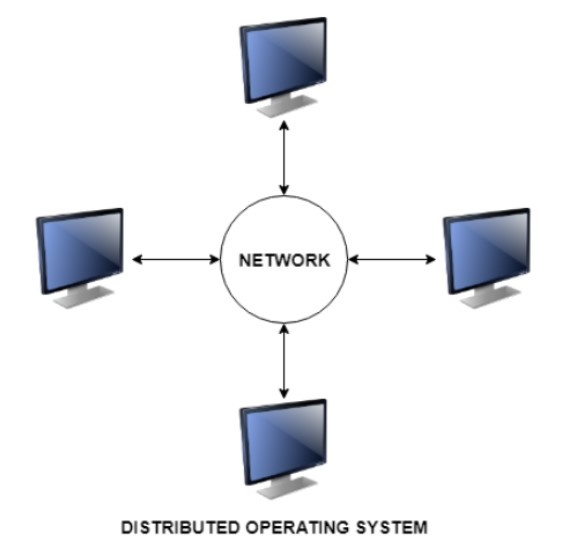
\includegraphics[scale=0.8]{sistemdistribusi1}
	\caption{Sistem Terdistribusi}
	\label{fig:sistemdistribusi1}
\end{figure}

\subsection{Manfaat Sistem Terdistribusi}
\noindent Berikut adalah manfaat penggunaan sistem terdistribusi:

\begin{itemize}
\item \textit{Horizontal scalability}\\
Sistem terdistribusi menawarkan kemampuan untuk melakukan pemrosesan komputasi skala besar pada big data dengan harga yang murah.

\item \textit{Reliability}\\
Sistem terdistribusi dapat diandalkan karena proses komputasi pada sistem terdistribusi bergantung pada banyaknya komputer yang saling berkomunikasi satu sama lain untuk mencapai tujuan yang sama.
 
\item \textit{Performance}\\
Sistem terdistribusi dapat menangani proses komputasi tugas secara efisien karena beban kerja sesungguhnya dibagi menjadi beberapa bagian dan tersebar di beberapa komputer. 
\end{itemize}

\subsection{Tantangan Sistem Terdistribusi} 
\noindent Berikut adalah tantangan pada sistem terdistribusi:

\begin{itemize}
\item Penjadwalan\\
Kekuatan komputasi ada batasnya, sehingga sistem terdistribusi harus dapat memutuskan pekerjaan mana yang harus dikerjakan lebih dulu.
\item Latensi\\
Dengan pertukaran data antara perangkat keras dan perangkat lunak menggunakan jalur komunikasi jaringan, sehingga nilai latensi menjadi sangat tinggi. 
\item Observasi\\
Ketika sistem terdistribusi menjadi kompleks, kemampuan pengamatan untuk memahami kegagalan pada sistem terdistribusi merupakan tantangan besar komputer. 
\end{itemize}

\section{Big Data}
\textit{Big data} adalah data yang besar dan kompleks sehingga tidak mungkin sistem tradisional dapat memproses dan bekerja pada lingkungan data yang besar secara maksimal. Data dapat dikategorikan sebagai data besar berdasarkan berbagai faktor. Konsep utama yang umum dalam semua faktor  adalah jumlah data. \\

\noindent Berikut adalah karakteristik 5V pada \textit{big data}:

\begin{itemize}
\item \textit{Volume}\\
\textit{Volume} mengacu pada jumlah data yang sangat besar. Data tumbuh begitu besar sehingga sistem komputasi tradisional tidak lagi dapat menanganinya seperti yang kita inginkan.

\item \textit{Velocity}\\
\textit{Velocity} mengacu pada kecepatan di mana data dihasilkan. Setiap hari, sejumlah besar data dihasilkan, disimpan, dan dianalisis. Data dihasilkan dengan kecepatan kilat di seluruh dunia. Teknologi \textit{big data} memungkinkan untuk mengeksplorasi data, saat data itu dihasilkan.

\item \textit{Variety}\\
\textit{Variety} mengacu pada berbagai jenis data. Data terutama dikategorikan ke dalam data terstruktur dan tidak terstruktur. Faktanya, lebih dari 75 persen data dunia ada dalam bentuk yang tidak terstruktur. 

\item \textit{Veracity}\\
\textit{Veracity} mengacu pada kualitas data. Ketika menyimpan beberapa data yang besar, apabila tidak ada gunanya di masa depan, maka membuang-buang sumber daya untuk menyimpan data tersebut. Jadi, kita harus memeriksa kepercayaan data sebelum menyimpannya. 

\item \textit{Value}\\
\textit{Value} adalah bagian terpenting dari big data. Organisasi menggunakan data besar untuk menemukan nilai informasi baru. Menyimpan sejumlah besar data sampai pada ekstraksi informasi yang bermakna dari sekumpulan data tersebut.
\end{itemize}

\noindent \textit{Big data} memerlukan teknologi tertentu untuk melakukan komputasi. Pada bagian selanjutnya akan dijelaskan konsep-konsep terkait penggunaan \textit{framework} beserta komponen-komponen penting pada \textit{framework} tersebut terkait komputasi pada lingkungan \textit{big data}. \textit{Framework} tersebut antara lain Hadoop dan Spark. Masing-masing \textit{framework} akan diteliti lebih lanjut, untuk dipilih pada penelitian ini berdasarkan kecepatan waktu komputasi.

\section{Hadoop}
Hadoop adalah \textit{framework} yang memanfaatkan beberapa komputer untuk menyelesaikan masalah yang melibatkan volume data sangat besar. Hadoop memecah input dari pengguna menjadi beberapa blok data dan masing-masing blok data diproses menggunakan konsep \textit{MapReduce} di mana data akan diproses secara paralel pada sistem terdistribusi. 

\subsection{HDFS}
HDFS adalah sistem \textit{file} terdistribusi pada Hadoop yang menyediakan penyimpanan data yang handal dengan mendukung partisi data dan toleran terhadap kesalahan pada hardware. HDFS bekerja erat dengan MapReduce dengan mendistribusikan penyimpanan dan perhitungan di seluruh \textit{cluster} dengan menggabungkan seluruh penyimpanan data menjadi terpusat.

\subsection{MapReduce}
\textit{MapReduce} adalah model pemrograman untuk memproses data berukuran besar secara terdistribusi dan paralel pada cluster yang terdiri atas banyak komputer. Dalam memproses data, secara garis besar, MapReduce dibagi menjadi dua jenis proses yaitu map dan reduce. Setiap fase memiliki pasangan key-value sebagai input dan output. Kedua jenis proses ini didistribusikan ke setiap komputer dalam suatu cluster dan berjalan secara paralel tanpa saling bergantung satu sama lain.

\begin{figure}[H]
	\centering
	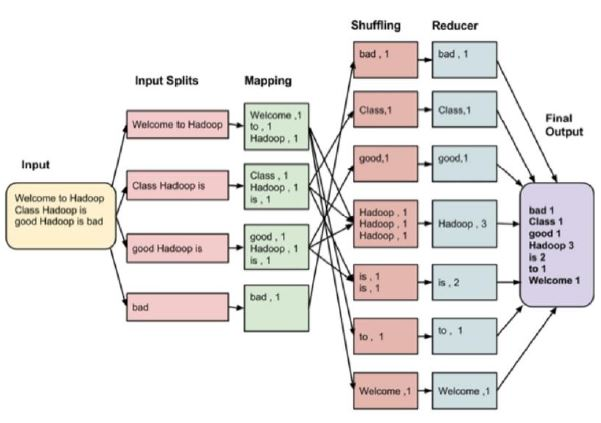
\includegraphics[scale=1.1]{MapReduceImage2}
	\caption{Proses Komputasi pada MapReduce}
	\label{fig:MapReduceImage}
\end{figure}

\noindent Berikut adalah penjelasan masing-masing tahapan pada MapReduce:

\begin{itemize}
\item Input\\
Pada tahap ini, model MapReduce menerima input data secara utuh dari file text/CSV.

\item Input Splits
Pada tahap ini, model MapReduce akan memecah input data menjadi blok-blok data dan disebarkan ke seluruh cluster.

\item \textit{Mapping}\\
\textit{Mapping} bertujuan untuk memetakan blok-blok data ke dalam pasangan <\textit{key},\textit{value}>. Key,Value pada contoh ini adalah jenis kata dan jumlah jenis kata pada sebuah blok data.

\item Shuffling\\
Shuffling bertujuan untuk mengirim data dari Mapping ke Reducer, agar data dengan key yang sama akan dikelompokan dan diolah oleh Reducer yang sama

\item Reducer \\
Reducer bertujuan sebagai proses penggabungan key,value dari proses shuffling untuk dihitung dan dikembalikan sebagai sebuah output

\item Output\\
Pada tahap ini, pemodelan MapReduce telah selesai. Output siap untuk ditulis pada file maupun ditampilkan pada console.

\end{itemize}

\newpage
\section{Spark} 
\label{sec:konsep_spark}
Spark adalah teknologi komputasi \textit{cluster} yang dirancang untuk komputasi cepat. Spark adalah paradigma pemrosesan data berukuran besar yang dikembangkan oleh para peneliti \textit{University of California di Berkeley}. Spark adalah alternatif dari Hadoop MapReduce untuk mengatasi keterbatasan pemrosesan input output yang tidak efisien pada disk, dengan menggunakan memori. Fitur utama Spark adalah melakukan komputasi di dalam memori sehingga waktu komputasi menjadi lebih singkat dibandingkan waktu komputasi di dalam \textit{disk}.
\\\\
Berikut adalah karakteristik dari Spark:

\begin{itemize}
\item Kecepatan\\
Spark adalah alat komputasi \textit{cluster} tujuan umum. Ini menjalankan aplikasi hingga 100 kali lebih cepat dalam memori dan 10 kali lebih cepat pada \textit{disk} daripada Hadoop. Spark mengurangi jumlah operasi baca/tulis pada \textit{disk} dan menyimpan data dalam memori.

\item Mudah untuk diatur\\	
Spark dapat melakukan pemrosesan \textit{batch}, analisis data secara interaktif, \textit{machine learning}, dan \textit{streaming data}. Semuanya pemrosesan tersebut dikerjakan pada satu komputer yang sama. Fungsi ini menjadikan Apache Spark sebagai mesin analisis data yang lengkap. 

\item Analisis secara \textit{real-time}\\
Spark dapat dengan mudah memproses data \textit{real-time}, misalnya \textit{streaming} data secara \textit{real-time} untuk ribuan peristiwa/detik. Contoh dari sumber \textit{streaming} data adalah Twitter, Facebook, Instagram. \textit{Streaming} data dapat diproses secara efisien oleh Spark.
\end{itemize}

\subsection{Ekosistem Spark}
\begin{figure}[H]
	\centering
	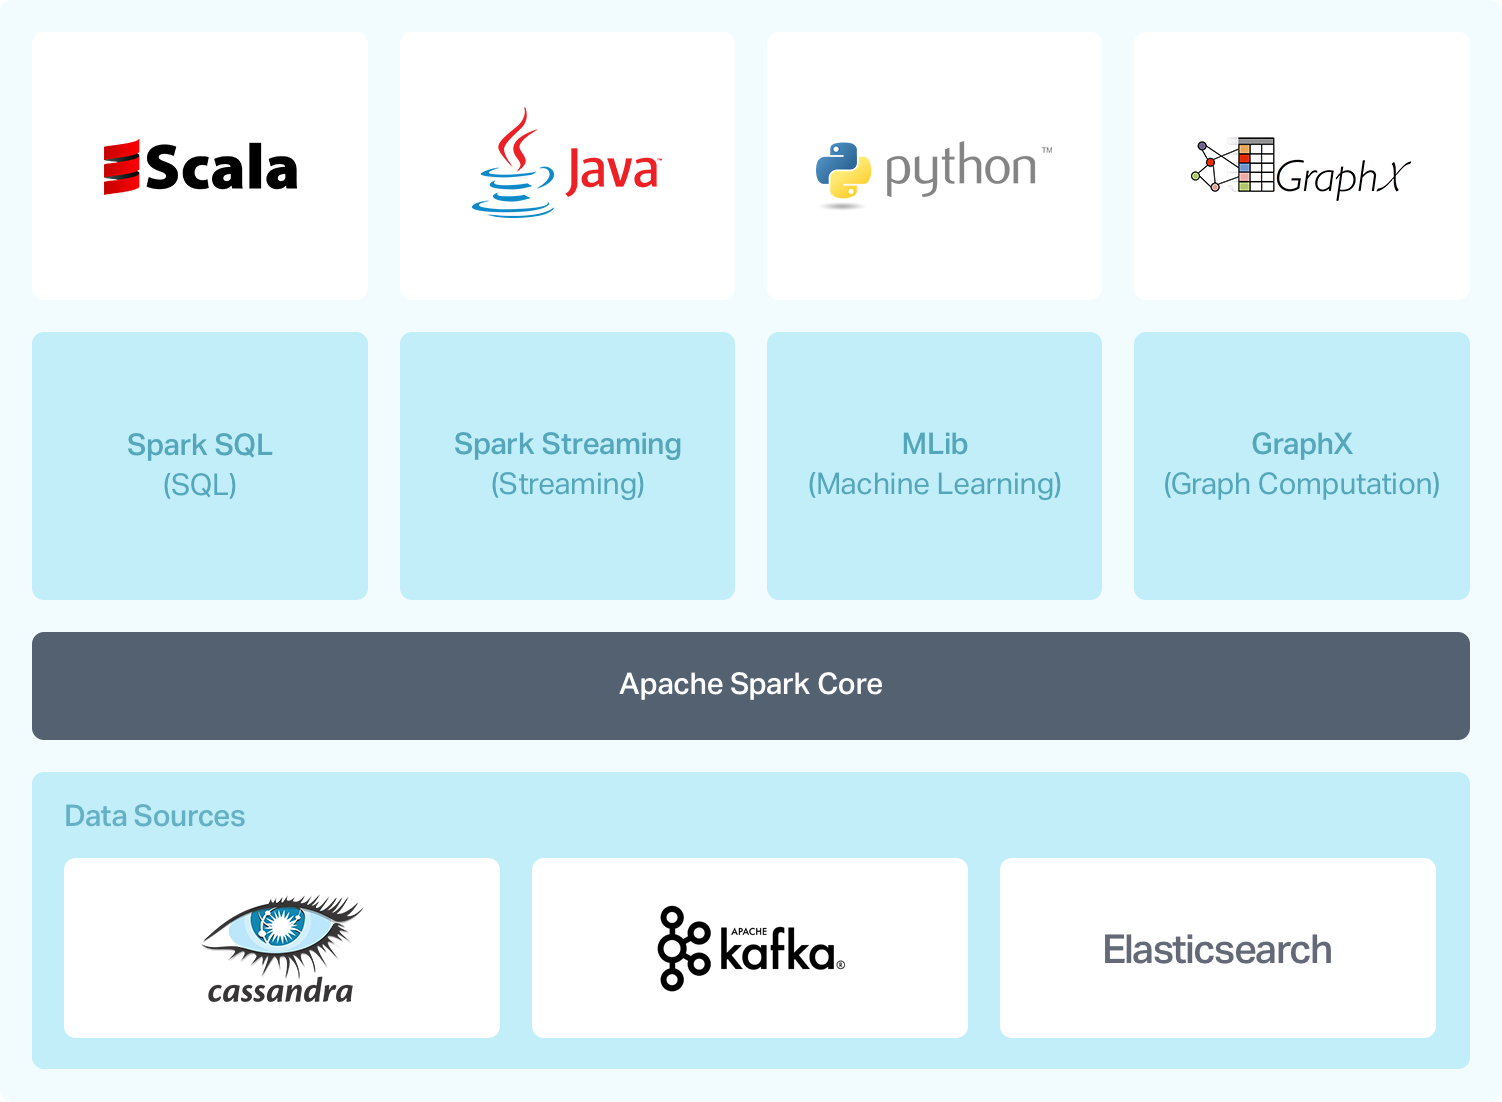
\includegraphics[scale=0.18]{spark_ecosystem}
	\caption{Ekosistem Spark}
	\label{fig:spark_ecosystem}
\end{figure}
Gambar \ref{fig:spark_ecosystem} menunjukan bahwa Spark bekerja sama dengan teknologi \textit{big data} lain untuk memenuhi berbagai macam kebutuhan dalam pengolahan \textit{big data}. Masing-masing warna pada Gambar \ref{fig:spark_ecosystem} mewakili jenis teknologi yang dipakai pada Spark. Spark SQL, Spark Streaming, Spark MLlib adalah \textit{library} tambahan pada Spark. Cassandra, Kafka, dan ElasticSearch adalah \textit{framework} untuk melakukan pengumpulan data secara \textit{streaming}. Scala, Java, dan Python adalah bahasa pemrograman yang dapat digunakan pada Spark.

\subsection{Arsitektur Spark}
\label{sec:arsitektur_spark}
\begin{figure}[H]
	\centering
	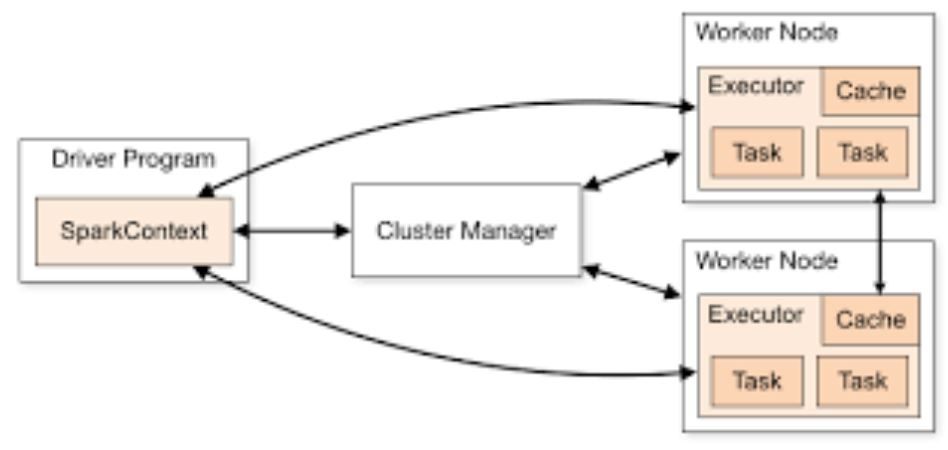
\includegraphics[scale=0.4]{arsitektur_spark2}
	\caption{Arsitektur Spark}
	\label{fig:arsitektur_spark2}
\end{figure}

Berdasarkan Gambar \ref{fig:arsitektur_spark2}, berikut adalah beberapa hal penting terkait arsitektur Spark:

\begin{itemize}

\item \textit{Driver Program} bertugas untuk menjalankan \textit{Object main} pada \textit{master node}. \textit{Driver Program} adalah tempat dimana \textit{Spark Context} dibuat.

\item \textit{Spark Context} bertugas untuk menghubungkan pengguna dengan \textit{cluster}. \textit{Spark Context} juga digunakan untuk membuat RDD, \textit{accumulator}, dan \textit{broadcast variable}.

\item \textit{Cluster Manager} bertugas untuk mengatur sumber daya pada sebuah \textit{cluster}.

\item \textit{Executor} membantu memantau proses-proses yang berjalan pada \textit{worker node} dan bertanggung jawab untuk mengerjakan \textit{task} yang diberikan.

\item \textit{Task} adalah satuan kerja pada Spark yang berisi perintah-perintah fungsi yang diserialisasi.

\end{itemize}


\subsection{Jenis Instalasi pada Spark}
\label{sec:instalasi_spark}
\begin{figure}[H]
	\centering
	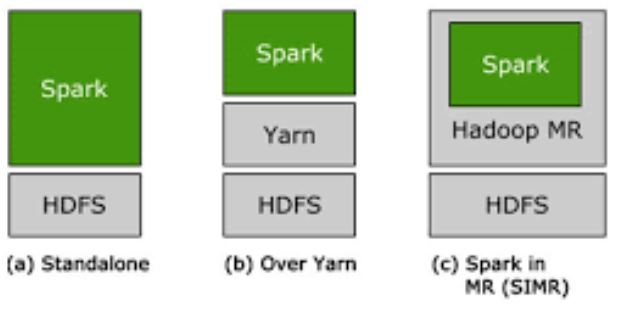
\includegraphics[scale=0.5]{arsitektur_spark}
	\caption{Arsitektur Spark}
	\label{fig:arsitektur_spark}
\end{figure}

Berdasarkan Gambar \ref{fig:arsitektur_spark}, berikut adalah jenis-jenis instalasi pada Spark:

\begin{itemize}
\item \textit{Standalone}\\  
Spark berdiri diatas HDFS Hadoop. Spark memungkinkan untuk mengakses data pada HDFS Hadoop untuk membaca input dan menulis output.

\item \textit{Hadoop Yarn}\\
Spark dapat berjalan pada Hadoop Yarn tanpa memerlukan instalasi atau meminta hak akses \textit{root} apapun. Hadoop Yarn membantu integrasi Spark pada ekosistem Hadoop.

\item \textit{Spark In MapReduce} (SIMR)\\ 
SIMR digunakan untuk menjalankan pekerjaan Spark secara independen. Jenis instalasi ini sudah tidak lagi berlaku untuk Spark versi 2.0
\end{itemize}

\subsection{Resilient Distibuted Datasets (RDD)}
\label{sec:rdd}
\par RDD adalah kumpulan partisi terdistribusi yang disimpan dalam memori atau \textit{disk} pada beberapa \textit{cluster}. RDD tersebar menjadi beberapa partisi,  sehingga partisi tersebut dapat disimpan dan diproses pada komputer yang berbeda. \\

\noindent Berikut adalah beberapa karakteristik yang dimiliki RDD:

\begin{itemize}

\item \textit{Lazy evaluation}: operasi pada Spark hanya akan dilakukan ketika memanggil fungsi \textit{Action}.

\item \textit{Immutability}: data yang disimpan dalam RDD tidak dapat diubah nilainya. 

\item \textit{In-memory computation}: RDD menyimpan data secara langsung dalam memori.

\item \textit{Partitioning}: dapat membagi pekerjaan RDD pada beberapa komputer.

\end{itemize}

\noindent Berikut adalah jenis operasi pada RDD:

\begin{itemize}
\item Fungsi \textit{Transformation}\\
Fungsi \textit{transformation} dilakukan secara \textit{lazy}, sehingga hanya akan dikerjakan apabila dipanggil pada fungsi \textit{action}. Fungsi \textit{transformation} pada RDD akan dijelaskan pada tabel dibawah ini.\\

\begin{tabular}{|l|p{10cm}|}
\hline 
\rule[-1ex]{0pt}{2.5ex} Fungsi & Deskripsi \\ 
\hline 
\rule[-1ex]{0pt}{2.5ex} map() & Mengembalikan RDD baru dengan menerapkan fungsi pada setiap elemen data \\ 
\hline 
\rule[-1ex]{0pt}{2.5ex} filter() & Mengembalikan RDD baru yang dibentuk dengan memilih elemen-elemen sumber di mana fungsi mengembalikan true \\ 
\hline 
\rule[-1ex]{0pt}{2.5ex} reduceByKey() & Menggabungkan nilai-nilai kunci menggunakan fungsi \\ 
\hline 
\end{tabular} 

\vspace{0.2cm}

\item Fungsi \textit{Action}\\
Fungsi \textit{Action} adalah operasi yang mengembalikan nilai output ke dalam terminal atau melakukan penulisan data pada sistem penyimpanan eksternal. Fungsi \textit{Action} memaksa evaluasi pada RDD yang akan dipanggil, untuk menghasilkan output. Fungsi \textit{Action} pada RDD akan dijelaskan pada tabel dibawah ini.\\

\begin{tabular}{|l|p{10cm}|}
\hline 
\rule[-1ex]{0pt}{2.5ex} Fungsi & Deskripsi \\ 
\hline 
\rule[-1ex]{0pt}{2.5ex} count() & Mendapat jumlah elemen data dalam RDD \\ 
\hline 
\rule[-1ex]{0pt}{2.5ex} reduce() & Agregat elemen data ke dalam RDD dengan mengambil dua argumen dan mengembalikan satu \\ 
\hline 
\rule[-1ex]{0pt}{2.5ex} foreach(operation) & Menjalankan operasi untuk setiap elemen data dalam RDD \\ 
\hline 
\end{tabular} 
\end{itemize}

\subsection{\textit{Dataframe}}
\label{sec:dataframe}
\textit{Dataframe} adalah kumpulan data yang didistribusikan, disusun dalam baris dan kolom. Setiap kolom dalam \textit{Dataframe} memiliki nama dan tipe terkait. \textit{Dataframe} mirip dengan tabel database tradisional, yang terstruktur dan ringkas. Dengan menggunakan \textit{Dataframe}, kueri SQL dapat dengan mudah diimplementasi pada \textit{big data}.\\

\noindent Berikut adalah beberapa karakteristik yang dimiliki \textit{Dataframe}:
\begin{itemize}
\item Terdiri atas baris dan kolom seperti tabel.
\item Memiliki skema untuk penyimpanan data
\item Data yang dapat disimpan berupa numerik dan kategorikal.
\item Dapat dilakukan pemrosesan kueri SQL.
\end{itemize}

\newpage
\subsection{Komponen Spark}
\label{sec:komponen_spark}
Komponen Spark adalah library tambahan pada Spark untuk melakukan proses komputasi pada lingkungan big data berdasarkan jenis-jenis kebutuhan pengolahan data. Berikut adalah penjelasan singkat mengenai komponen pada Spark:

\begin{itemize}
\item Spark Core \\
Spark Core adalah \textit{library} Spark yang berisi fungsionalitas dasar Spark, termasuk komponen untuk penjadwalan tugas, manajemen memori, pemulihan kesalahan, dan berinteraksi dengan sistem penyimpanan. Spark Core menyediakan komputasi pada memori, fungsi \textit{action} dan \textit{transformation} untuk mengolah RDD.

\item Spark SQL  \\
Spark SQL memungkinkan pemrosesan kueri SQL pada lingkungan big data. Spark SQl menyediakan fungsi untuk menghitung nilai statistik dasar seperti \textit{mean, median, modus}, nilai maksimum dan nilai minimum.

\item Spark Streaming \\
Spark Streaming adalah salah satu komponen Apache Spark, yang memungkinkan Spark dapat memproses data \textit{streaming} secara \textit{real-time}. Spark Streaming menyediakan API untuk memanipulasi aliran data yang cocok dengan RDD. Hal ini memungkinkan analisis data untuk beralih melalui sumber aplikasi yang memberikan data secara \textit{real-time}. 

\item
Spark MLlib \\
Spark MLlib adalah \textit{library} Spark yang berisi fungsionalitas yang umum digunakan pada \textit{machine learning}. Untuk mengimplementasikan teknik \textit{data mining} pada lingkungan \textit{big data} dibutuhkan \textit{library} Spark MLlib. Spark MLlib menyediakan berbagai jenis algoritma \textit{machine learning} termasuk klasifikasi dan pengelompokan/\textit{clustering}.
\end{itemize}

\section{Spark MLlib}
\label{sec:konsep_spark_mllib}
Spark MLlib adalah library pembelajaran mesin berdasarkan komputasi secara paralel. MLlib terdiri dari algoritma pembelajaran umum seperti klasifikasi, pengelompokan/\textit{clustering}. Secara garis besar, MLlib melakukan data \textit{preprocessing}, pelatihan model, dan membuat prediksi.

\subsection{Machine Learning pada Spark MLlib}
\label{sec:ml_sparkmllib}
\begin{figure}[H]
	\centering
	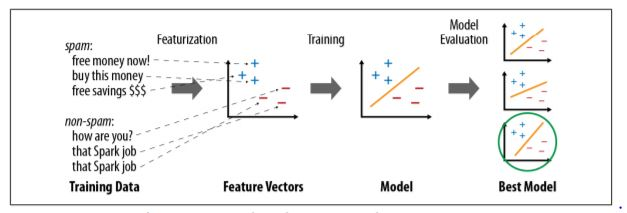
\includegraphics[scale=0.8]{machinelearningmllib}
	\caption{Tahapan Pembelajaran Machine Learning}
	\label{fig:machinelearningmllib}
\end{figure}

\textit{Machine learning} bertujuan membuat prediksi label/kelompok data berdasarkan jenis model yang dipakai. Pemodelan \textit{machine learning} mencakup model dari\textit{data mining}. Pemodelan \textit{machine learning} membutuhkan input berupa vektor fitur. Vektor fitur adalah nilai masing-masing atribut yang digunakan pada pelatihan data. 

\noindent Gambar \ref{fig:machinelearningmllib} adalah tahapan \textit{machine learnin}g pada Spark MLlib, berikut adalah penjelasan singkat dari masing-masing tahapan:

\begin{enumerate}

\item \textit{Featurization}\\
Pemodelan \textit{machine learning} hanya dapat menerima input berupa vektor. Oleh karena itu, nilai atribut pada tabel akan diubah ke representasi numerik dalam bentuk vektor. 
 
\item \textit{Training}\\
Pemodelan \textit{machine} learning melakukan pelatihan agar model yang dipakai memberikan hasil yang tepat untuk menentukan label atau kelompok data. Oleh karena itu, pemodelan \textit{machine learning} memerlukan pelatihan model beberapa kali untuk mendapatkan model terbaik.

\item \textit{Model Evaluation}\\
Pada akhir pelatihan, model yang terbentuk dapat diputuskan baik atau tidak melalui perhitungan nilai akurasi. Semakin besar nilai akurasi, maka model dapat digunakan untuk memprediksi nilai label atau kelompok data secara tepat.
\end{enumerate}

\subsection{Tipe Data pada Spark MLlib}
Seperti yang sudah dijelaskan pada bagian \ref{sec:ml_sparkmllib}, pemodelan \textit{machine learning} menerima input berupa vektor fitur. Tipe data yang disediakan pada Spark MLlib terdiri dari beberapa jenis yaitu vektor, \textit{labeledpoint}, dan \textit{various model class}. \\

\noindent Berikut adalah beberapa jenis tipe data pada Spark MLlib:

\begin{itemize}
\item Vektor\\
Vektor terdiri dari dua jenis yaitu vektor dense dan vektor sparse. Kelas vektor berada pada \textit{package} mllib.linalg.Vectors. Gambar \ref{fig:vektor} adalah contoh vektor dense dan vektor sparse:

\begin{figure}[H]
	\centering
	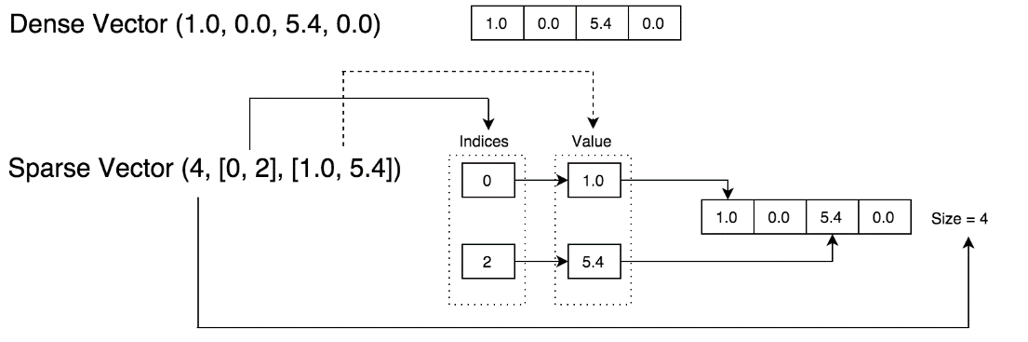
\includegraphics[scale=0.6]{vektor}
	\caption{Contoh Vektor Dense dan Sparse}
	\label{fig:vektor}
\end{figure}

\begin{itemize}

\item Vektor \textit{dense}\\
Vektor \textit{dense} adalah vektor yang menyimpan setiap nilai fitur dataset. Jumlah elemen pada vektor \textit{dense} akan memiliki jumlah yang sama dengan jumlah fitur pada dataset.

\item Vektor \textit{sparse}\\
Vektor \textit{sparse} adalah vektor yang menyimpan setiap nilai fitur yang bukan nol pada dataset, sehingga jumlah elemen yang disimpan pada vektor \textit{sparse} lebih sedikit dibandingkan dengan jumlah elemen yang disimpan pada vektor \textit{dense}. 

\end{itemize}

\item \textit{LabeledPoint}\\
\textit{LabeledPoint} digunakan pada algoritma \textit{supervised learning} yaitu klasifikasi dan regresi. Kelas \textit{LabeledPoint} terletak pada \textit{package} mllib.regress.

\item \textit{Various Model class}\\
\textit{Various Model classes} adalah tipe data yang dihasilkan dari pemodelan \textit{machine learning}. Tipe data ini memiliki fungsi predict() untuk melakukan prediksi label dan kelompok data.

\end{itemize}

\subsection{\textit{Data Mining} pada Spark MLlib}
Data mining pada Spark MLlib menggunakan tahapan pemodelan pada \textit{machine learning} yang dijelaskan pada bagian \ref{sec:ml_sparkmllib} untuk menghasilkan tabel hasil pengelompokan dan klasifikasi. Pada bagian ini akan dijelaskan parameter dari pemodelan Spark MLlib.

\subsubsection{\textit{Naive Bayes}}
\label{sec:naivebayes_mllib}
\textit{Naive Bayes} menjadi pemodelan klasifikasi yang umum digunakan. \textit{Naive Bayes} dapat dilatih dengan sangat efisien karena prosesnya hanya menghitung probabilitas bersyarat. \textit{Naive Bayes} memiliki parameter masukan sebagai berikut:
 
\begin{itemize}
\item \textit{randomSplit} adalah membagi \textit{training} dan \textit{test} data berdasarkan persentase.
\item \textit{setModelType} adalah memilih model yang tersedia (\textit{multinomial/bernoulli})
\item \textit{setLabelCol} adalah memilih jenis atribut yang menjadi label kelas.
\end{itemize}

\subsubsection{\textit{K-Means}}
\label{sec:kmeans_mllib}
\textit{K-means} menjadi pemodelan pengelompokan/\textit{clustering} yang paling umum digunakan untuk mengelompokkan titik-titik data menjadi sejumlah kelompok yang telah ditentukan. \textit{K-means} memiliki parameter masukan sebagai berikut:

\begin{itemize}
\item \textit{k} adalah jumlah cluster yang diinginkan. 
\item \textit{maxIterations} adalah jumlah iterasi maksimum yang harus dijalankan.
\item \textit{initializationMode} menentukan inisialisasi centroid secara acak.
\item \textit{initializationSteps} menentukan jumlah langkah dalam algoritma \textit{k-means}.
\item \textit{initialModel} adalah menentukan nilai centroid saat inisialisasi.
\end{itemize}

\section{Scala}
\label{sec:scala}
Scala adalah bahasa pemrograman berbasi open source, dibuat oleh Profesor Martin Odersky. Scala adalah bahasa pemrograman multi-paradigma dan mendukung paradigma fungsional serta berorientasi objek. Untuk pengembangan Spark, penulisan sintaks Scala dianggap produktif untuk mengimplementasikan kode program. Pemrograman pada Scala mempertahankan prinsip keseimbangan antara produktivitas pengembangan program dan kinerja program. Pemrograman pada Scala tidak serumit pemrograman pada Java. Satu baris kode program pada Scala dapat menggantikan 20 hingga 25 baris kode Java. Karena alasan terbut, Scala menjadi bahasa pemrograman yang sangat diminati untuk melakukan pemrosesan \textit{big data} pada Spark.

\section{Scala Swing} 
Scala Swing adalah program berbasis \textit{Graphical User Interface} (GUI) sehingga memiliki perbedaan dengan program Spark yang dieksekusi dengan terminal. Scala Swing bertujuan untuk memberi tampilan program sehingga hasil program diharapkan menjadi lebih interaktif. Scala menyediakan akses langsung terhadap kelas GUI pada Java menggunakan \textit{library} Scala Swing.  Dengan menggunakan Scala, penggunaan Scala Swing dapat memenuhi kebutuhan perancangan \textit{User Interface} melalui berbagai macam komponen GUI pada umumnya. Gambar \ref{fig:swing_example} adalah contoh implementasi GUI sederhana pada Scala Swing.
\begin{figure}[H]
	\centering
	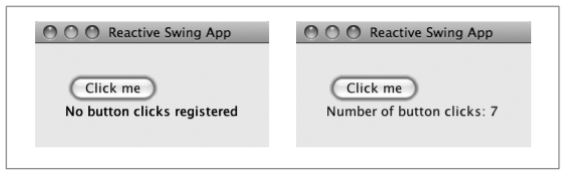
\includegraphics[scale=0.9]{swing_example}
	\caption{GUI Sederhana pada Scala Swing}
	\label{fig:swing_example}
\end{figure}


\subsection{Panel dan Layout}
\textit{Panel} adalah tempat untuk menampilkan semua komponen GUI dengan beberapa aturan tata letak yang harus dipenuhi. Salah satu bagian tersulit pada perancangan aplikasi berbasis GUI adalah mengatur penempatan layout dengan benar. \textit{Layout} terdiri dari beberapa komponen GUI seperti \textit{Frame, Panel, Label} atau \textit{Button}. Masing-masing komponen GUI pada \textit{layout} memiliki nilai properti sendiri (warna, ukuran, posisi) yang dapat diatur secara manual.

\subsection{Handling Event}
\textit{Handling event} adalah perkerjaan yang dilakukan masing-masing komponen. Komponen akan menerima aksi langsung dari pengguna aplikasi. Mekanisme ini dikenal sebagai \textit{handling event}, yang dieksekusi ketika suatu peristiwa terjadi. \textit{Handling event} memiliki \textit{listener}. \textit{Listener} adalah sebuah komponen memberi tahu sebuah aksi kepada komponen tertentu. \textit{Listener} harus dibuat untuk masing-masing objek \textit{handling event}. 

\section{Format Penyimpanan Data}
\label{theory:csv}
Spark dapat melakukan aksi membaca dan menulis pada data terstruktur dan semi terstruktur. Contoh data terstruktur yang umum digunakan adalah CSV, sedangkan contoh data semi terstruktur yang umum digunakan adalah JSON. Berikut adalah penjelasan lengkap mengenai format penyimpanan data CSV dan JSON.

\subsection{CSV}
CSV \textit{(Comma Separated Values)} menjadi format yang sangat umum digunakan untuk menyimpan nilai pada tabel data yang terstruktur. CSV menggunakan format ekstensi (.csv) saat berdiri sendiri. Hasil penyimpanan dengan format CSV umum digunakan untuk menyimpan data saat ingin menyimpan tabel dari basis data. CSV memisahkan nilai atribut yang satu dengan yang lainnya menggunakan tanda koma. CSV dapat memisahkan data yang satu dengan data lainnya berdasarkan penempatan data pada baris yang berbeda. Listing \ref{lst:lst_csv} adalah contoh format penyimpanan CSV.

\begin{lstlisting}[basicstyle=\ttfamily, frame=single,
	columns=fullflexible, keepspaces=true, breaklines=true, label=lst:lst_csv, caption=Format Penyimpanan CSV]
age,workclass,zip,education,year_of_education,marital_status,occupation
39,State-gov,77516,Bachelors,13,Never-married,Adm-clerical
50,Self-emp-not-inc,83311,Bachelors,13,Married-civ-spouse,Exec-managerial
38,Private,215646,HS-grad,9,Divorced,Handlers-cleaners
53,Private,234721,11th,7,Married-civ-spouse,Handlers-cleaners
28,Private,338409,Bachelors,13,Married-civ-spouse,Prof-specialty
37,Private,284582,Masters,14,Married-civ-spouse,Exec-managerial
49,Private,160187,9th,5,Married-spouse-absent,Other-service
52,Self-emp-not-inc,209642,HS-grad,9,Married-civ-spouse,Exec-managerial
\end{lstlisting}

\subsection{JSON}
JSON \textit{(JavaScript Object Notation)} adalah format untuk pertukaran data. JSON menggunakan format ekstensi (.json) saat berdiri sendiri. JSON diturunkan dari bahasa pemrograman JavaScript. Walaupun diturunkan dari bahasa pemrograman lain, JSON tidak bergantung pada bahasa pemrograman apapun. Oleh karena itu, format JSON sangat mudah dipakai untuk pertukaran data antar bahasa pemrograman. JSON memiliki format penyimpanan \textit{key-value} seperti pada Listing \ref{lst:lst_json}. JSON menyimpan enam jenis tipe data yaitu \textit{string, number, object, array, boolean, null}. Menulis format JSON dalam beberapa baris akan lebih mudah dibaca terutama saat datanya sudah banyak. 

\begin{lstlisting}[basicstyle=\ttfamily, frame=single,
	columns=fullflexible, keepspaces=true, breaklines=true, label=lst:lst_json, caption=Format Penyimpanan JSON]
{
    "firstName": "Rack",
    "lastName": "Jackon",
    "gender": "man",
    "age": 24,
    "address": {
        "streetAddress": "126",
        "city": "San Jone",
        "state": "CA",
        "postalCode": "394221"
    },
    "phoneNumbers": [
        { "type": "home", "number": "7383627627" }
    ]
}
\end{lstlisting}








